% chktex-file 1   user-defined macros (\NumPrimes etc.) terminated with space is correct
% chktex-file 3   [0,1] interval notation in math mode is correct
% chktex-file 8   en-dash compounds are correct academic usage
% chktex-file 12  interword spacing in captions is intentional
% chktex-file 13  intersentence spacing is a style choice
% chktex-file 24  \label on own line is standard practice
% chktex-file 36  acronym parentheses (e.g. Top-$K$) need no leading space
% chktex-file 38  American-style punctuation inside closing quotes is correct
\chapter{Predictive Modeling for Supply-Link Discovery}
\label{chap:link-prediction}

%========================
% Chapter 2
%========================
%========================
% Section 2.0
%========================

This section treats supply-chain visibility as a predictive problem. The Department of Defense depends on multi-tier, global semiconductor supply chains whose upstream structures are only partially observable from public disclosures, so any rigorous assessment of continuity and integrity risk requires extending that view beyond what firms happen to report. FactSet's Supply Chain Relationships (SCR) graph is modeled as a positive--unlabeled link-prediction task: starting from a sparse set of disclosed supplier$\rightarrow$customer ties, the models estimate probabilistic scores for millions of undisclosed firm pairs. The aim is not to reconstruct the entire global production network, but to produce a high-precision set of inferred links that materially expands the map of DoD-relevant semiconductor dependencies. \S2.1 constructs a frozen, leakage-safe dataset for estimation; \S2.2 defines the shared candidate-pool ranking task and evaluation scorecard; and \S2.3--\S2.10 compare model families and robustness checks whose calibrated scores and operating points serve as the main outputs of this section and the inputs to Section~\ref{chap:dod-supply-chain}.

For readers primarily interested in the policy implications rather than the technical methodology: this section evaluates six families of link-prediction models---algorithms that score how likely two firms are to have an undisclosed supply relationship. The ensemble model that combines all six achieves approximately \CorePrecision\% measured precision (a conservative lower bound under positive--unlabeled labeling) with over 600$\times$ lift above random chance, meaning it identifies real supply links far more reliably than any single approach. The sections that follow document how those results were validated; the key outputs---predicted supply edges with confidence scores---are carried forward into Section~\ref{chap:dod-supply-chain}'s network construction.

The starting point for this section is FactSet's Supply Chain Relationships (SCR) dataset, an analyst-curated record of inter-firm supplier--customer ties drawn from corporate disclosures \parencite{factset_supply_2024}. SCR captures relationships that companies explicitly name in press releases, investor relations materials, regulatory filings, and similar sources, and maps both parties to a global firm identifier space. Each record specifies a supplier, a customer, and effective dates for the relationship, yielding a directed, time-stamped catalogue of disclosed supplier$\rightarrow$customer links across sectors and regions \parencite{factset_supply_2024}. SCR serves as the disclosed layer. It provides the oriented edges, timestamps, and canonical firm identifiers used to define the observed graph and the set of positive labels for link prediction.

From these disclosures, a baseline supply graph is constructed on which all models in this section operate. After normalizing relationship events and deduplicating overlapping episodes, the full disclosure history spans approximately \NumFirms firms and about 1.2 million unique disclosed supplier$\rightarrow$customer pairs across all years. Each node is a canonical firm keyed to a stable FactSet entity identifier, and each edge indicates that at least one supplier$\rightarrow$customer episode has been disclosed between the two firms, with the underlying event history preserved in a separate table. The graph is global and cross-sector, but, by construction, it captures only ties that appear in public disclosures; undisclosed but operationally important relationships are absent. This disclosure-based snapshot at the training cutoff is denoted $\mathcal{G}_{T_0}$ and treated as the sparse, incomplete baseline on which the link-prediction models in this section are trained and evaluated, with the details of event processing, node indexing, temporal splits, and the construction of $\mathcal{G}_{T_0}$ set out in \S2.1.

Examining the graph's degree distribution makes the incompleteness of disclosure clear. Figure~\ref{fig:degree-hist} shows why the disclosure record undercovers the network. Here, the report defines degree as the number of distinct disclosed counterparties with which a firm is either a supplier or a customer. Most firms fall into the lowest-degree bin (e.g., 0--50 distinct partners), and the frequency of firms drops sharply as degree increases on a log-scale y-axis. This pattern is consistent with heavy-tailed degree distributions in complex networks \parencite{barabasi_emergence_1999}. Still, it is implausible as a full representation of real production systems, in which firms typically rely on multiple upstream and downstream ties and in which shocks propagate through dense webs of firm-to-firm connections \parencite{inoue_firm-level_2019}. A more credible interpretation is that SCR selectively records a subset of real relationships, with coverage skewed toward larger, more visible firms and away from smaller, private, and sub-tier suppliers \parencite{gopal_discovering_2021}. The observed degree pattern, therefore, indicates that SCR provides a partial, biased slice of the underlying production network rather than a complete map.

% -------------------------- Degree Histogram -----------------------
\begin{figure}[tbp]
  \centering
  \caption[\textit{Observed Degree Distribution}]{\textit{Observed Degree Distribution}}
  \label{fig:degree-hist}

  
\includegraphics[width=0.90\linewidth]{report/figures/fig_01_degree_histogram.pdf}

  {%
    \captionsetup{justification=raggedright,singlelinecheck=false}
    \caption*{\footnotesize \textit{Note}. The histogram shows a heavy-tailed structure with substantial mass at low degrees, indicating that most entities appear with only a single observed counterparty in disclosures. This sparsity is implausible for real supply chains and motivates link prediction to recover hidden connectivity. The y-axis is logarithmic to reveal the long tail. Counts reflect disclosed relationships only; non-disclosure does not imply non-existence.}
  }
\end{figure}

This pattern motivates a positive--unlabeled framing for the prediction problem. This section treats a supplier$\rightarrow$customer pair as a positive if it appears in SCR by a given cutoff date within the label horizon. A true negative is a pair of firms that have no supply relationship over that horizon, but such negatives are rarely observed in practice. Firms disclose their material counterparties, but they do not certify that all other firms are absent from their supply chains. Given that most firms in SCR have only a handful of disclosed partners, it is more reasonable to view missing edges as under-reported ties rather than as evidence of non-relationships. The analysis, therefore, treats undisclosed pairs as unlabeled rather than negative and models the task as learning from known positives against an unlabeled background \parencite{elkan_learning_2008,bekker_learning_2020}. Under this positive--unlabeled view, estimated precision is best interpreted as a conservative lower bound on the true fraction of real supply relationships among high-scoring predicted links \parencite{elkan_learning_2008,gopal_discovering_2021}.

Under these conditions, simply taking the SCR graph at face value would systematically understate connectivity and obscure sub-tier dependencies that matter for DoD risk. The core task in this section is therefore supply-link discovery: the pipeline uses the structure of $\mathcal{G}_{T_0}$ and firm-level attributes to assign scores to unlabeled supplier$\rightarrow$customer pairs and to identify those with a high probability of representing real but undisclosed relationships. This follows the link-prediction tradition in partially observed graphs, where network structure and node features are used to infer missing edges \parencite{liben-nowell_link_2003,lu_link_2011}. The aim is not to exhaustively reconstruct the global production network, but to produce a high-precision expansion of the disclosure-based graph that meaningfully extends the DoD's view of its supply chain.

Shipping data might seem like an alternative source of training labels, but it serves only as a complementary flow signal rather than as ground truth. FactSet's trade and shipping feeds are built from event-level bills of lading and related customs records, with strong coverage of U.S. maritime imports but much weaker coverage of domestic movements and non-maritime trade \parencite{factset_factset_2021, factset_factset_2025}. Entity names are often non-standard, many records reflect freight forwarders or logistics providers rather than ultimate counterparties, and resolving these strings to the canonical firm identifiers used in SCR is noisy. These features make shipping data valuable for corroborating predicted links and marking some inferred edges as observed material flows, but they also make it a problematic primary source of labels. This section, therefore, relies on SCR to define positives for link prediction and reserves shipping for later sections, where it augments the disclosure-based network with a separate observed material-flow layer.

The time-stamped structure of this data also supports treating link prediction as a temporal rather than purely static problem. Features are drawn from an observation window extending up to a cutoff time $t_1$, with the training snapshot at $T_0$ as a special case, while labels are defined in a future window that begins after $t_1$. A supplier$\rightarrow$customer pair is positive in a given horizon if it is first disclosed in that future window; otherwise, it remains unlabeled. This design respects temporal order, so no information from after $t_1$ enters features at or before $t_1$, and it supports horizon-specific evaluation, where models are evaluated on how well they anticipate links that appear 0--6, 6--12, or more months beyond $T_0$ \parencite{holme_temporal_2012}. \S2.1 formalizes the exact observation and label windows, timestamp fields, and horizon bins used to describe the construction of the frozen core dataset.

By the end of this section, the analysis has a single calibrated ensemble model that assigns probability-like scores to candidate supplier$\rightarrow$customer pairs. The ensemble is designed to do two things. First, the SCR disclosure graph highlights relationships between disclosed and non-disclosed firms. Second, at the boundary of that graph, it scores candidate links involving firms that are weakly represented or absent from the original training snapshot. In Section~\ref{chap:dod-supply-chain}, the ensemble is applied to DoD-relevant candidate pairs, its predictions are combined with the disclosed layer and observed shipping connections, and the resulting high-probability links expand the semiconductor supply-chain network examined in that section.

\S2.1 formalizes the link-prediction problem for DoD visibility. It describes how the analysis constructs the frozen core dataset, including event processing, node indexing, temporal splits, and the $T_0$ snapshot. \S2.2 defines the candidate-pool ranking task, introduces the main metrics (Hit@$K$, Recall@$K$, Precision@$K$, MRR, MAP, normalized Discounted Cumulative Gain (nDCG@100)), and outlines the structural and temporal slices that comprise the shared evaluation scorecard. \S2.3 presents classical graph heuristics computed on $\mathcal{G}_{T_0}$ as fast, transparent baselines. \S2.4--\S2.6 introduce the learned models: Node2Vec, a static unsupervised embedding method; supervised snapshot models (GraphSAGE and a two-tower architecture); and temporal models (Node2Vec-Temporal and a temporal graph neural network). \S2.7 turns to calibration, complementarity, and ensembling; \S2.8 and~\S2.9 report scorecard results and analyze operating points and precision-yield frontiers that translate scores into concrete edge selections. Finally, \S2.10 assesses robustness and reproducibility, discusses the limits of the modeling and data, and prepares the ground for the DoD-focused network construction in Section~\ref{chap:dod-supply-chain}.

%========================
% Section 2.1
%========================
\section{Dataset Construction}

This section describes how the pipeline turns FactSet's Supply Chain Relationships (SCR) disclosures into a training-ready graph dataset for link prediction. Starting from raw SCR rows, it constructs a canonical, time-stamped history of supplier--customer relationships and builds a stable firm index that assigns each FactSet entity a unique node identifier. On top of this foundation, temporally ordered training, validation, and test windows are defined, a train-time graph snapshot \(\mathcal{G}_{T_0}\) is constructed, and fixed candidate pools are precomputed that specify, for every supplier with at least one future disclosure, which potential customer models will rank. Finally, a node feature layer is built that captures firm attributes and structural position as of \(T_0\). For the empirical work in this report, these steps yield \NumEpisodes directed relationship episodes among \NumFirms firms over 2003--2025. The remainder of this section walks through these transformations in the order they are applied.

The pipeline begins by extracting the full history of disclosed supplier--customer relationships from FactSet's Supply Chain Relationships (SCR) database as of \SCRExtractionDate \parencite{factset_supply_2024}. This query returns \NumRawRows raw rows, each describing a single disclosure episode with a supplier identifier, a customer identifier, and start and end dates for the reported relationship. A minimum start date of January 1, 2000 is required to focus on the modern semiconductor and defense-relevant period rather than legacy relationships from earlier decades. The schema is then standardized by parsing the start and end dates into a common timestamp type and coercing all identifiers to strings. At this stage, the table is still a direct reflection of the underlying feed: it contains self-loops, exact duplicate rows, and overlapping episodes that reflect reporting artifacts rather than distinct economic relationships.

The pipeline normalizes these raw disclosures to construct a canonical history of supplier--customer relationships. First, 60 self-loops are dropped in which the same firm appears as both supplier and customer, since these do not add information about inter-firm dependencies. Second, 93{,}438 exact duplicates within supplier--customer pairs are removed, defined as rows with identical endpoints and identical start and end dates, so that each disclosed episode appears only once. Third, ``near-duplicates'' are addressed by comparing overlapping intervals within each pair and discarding a new interval if more than 30\% of its duration overlaps an already accepted interval, removing an additional 92{,}388 rows. In total these filters eliminate 185{,}886 rows and leave \NumEpisodes distinct relationship episodes. For each surviving event, open-ended relationships are closed at the run date to compute a non-negative duration, calendar fields such as year, month, and quarter are derived from the start date, and time is encoded in both absolute days since January 1, 1970, and relative days since the earliest observed start date. Finally, direction is fixed by mapping the supplier identifier to the customer identifier, thereby establishing a consistent supplier$\rightarrow$customer convention for the remainder of the section.

Next, the pipeline builds a stable index over the firms that appear in this canonical event history. Taking the union of all supplier and customer identifiers from the cleaned table yields \NumFirms distinct FactSet entities, each treated as its own canonical entity. An internal node identifier is then assigned by sorting the canonical IDs in ascending order and numbering them \(0,1,\dots,\NumFirmsMinusOne\). This produces a three-column mapping from raw identifier to canonical identifier to \(\mathit{node\_id}\) that is written once and reused everywhere else in the pipeline. A simple metadata record contains the node-ID range, the total number of entities, and a checksum over the mapping file, thereby making the index auditable. All subsequent artifacts, including temporal splits, adjacency matrices, features, and models, refer to firms only through these node identifiers, which gives a single, consistent node space for the rest of the report.

With a cleaned event history and a stable firm index in hand, the pipeline imposes an explicit temporal structure on the data. Rather than drawing random train-test splits, firm-firm relationships are treated as evolving and each event's start date is used to define chronological windows. The goal is to train models on past disclosures and evaluate them on future disclosures, mirroring how analysts would use predictions in practice. The observed time span is partitioned into three contiguous segments, allocating 70\% to training, 15\% to validation, and 15\% to testing based on event start dates \parencite{goodfellow_deep_2016,xu_inductive_2020}. Between these windows, \InterSplitGap-day gaps are inserted so that events near the boundaries are discarded rather than used as either features or labels. Introducing such gaps is a common strategy to reduce temporal leakage, particularly in settings where labels arrive over time, and non-events are treated as negatives \parencite{bekker_learning_2020}. This design reduces temporal leakage between splits and supports both static models that see only \(\mathcal{G}_{T_0}\) and temporal models that use the event sequence more directly.

In the empirical dataset, the observed event window runs from April 3, 2003, to June 9, 2025. Using the epoch-day field \(\mathit{ts}\), which records days since January 1, 1970, this corresponds to \(\mathit{ts}=12{,}145\) through \(\mathit{ts}=20{,}248\). Applying the 70/15/15 allocation with \InterSplitGap-day gaps yields three disjoint splits. The training window includes all events with \(\mathit{ts} \le 17{,}757\), that is, disclosures with start dates on or before \TrainCutoffDate. The validation window is defined by \(17{,}817 \le \mathit{ts} \le 18{,}972\), which corresponds to October 13, 2018, through December 11, 2021. The test window begins at \(\mathit{ts} \ge 19{,}032\), that is, February 9, 2022, onward. Events whose start dates fall within the two \InterSplitGap-day buffer bands are discarded rather than used in any split, removing 24{,}358 events. The resulting splits contain 702{,}778 training edges, 354{,}979 validation edges, and 669{,}797 test edges. The training set covers 65{,}816 distinct sources and 98{,}584 distinct destinations, the validation set covers 49{,}778 sources and 80{,}809 destinations, and the test set covers 78{,}860 sources and 154{,}717 destinations, with all node identifiers drawn from the same 0--\NumFirmsMinusOne index.

On this temporal backbone, the pipeline constructs a train-time graph snapshot \(\mathcal{G}_{T_0}\) that represents the supply chain as it is known at the end of the training window. Starting from the training split, all edges \((\mathit{src\_id}, \mathit{dst\_id})\) are read, every node identifier is verified to lie in the global index range \(0\)-\(\NumFirmsMinusOne\), and duplicates are collapsed so that each directed pair appears at most once. A directed compressed sparse row (CSR) matrix of shape \(\NumFirms \times \NumFirms\) is then built, with a 1 wherever there is at least one train-time disclosure from supplier \(\mathit{src\_id}\) to customer \(\mathit{dst\_id}\). In this dataset, the resulting snapshot contains \TrainEdges unique directed edges, capturing all relationships disclosed through \TrainCutoffDate. From this CSR representation, node-level out- and in-degree vectors are derived and, for efficiency in later steps, a CSC transpose, a symmetrized undirected adjacency, and a small neighbor cache are optionally materialized. This snapshot contains no information from the validation or test periods and serves as the base graph for structural features and for models that assume a static network view at \(T_0\).

To evaluate models on a realistic search space, fixed candidate pools are defined for the validation and test splits. For each supplier node with at least one future disclosure, models rank not over all \(O(N^2)\) possible customers but over a smaller, structured set of plausible partners. Concretely, a pool of at most 5{,}000 candidate destinations is precomputed for every source with at least one positive edge in a split. Each pool always contains all known positives for that source in the relevant horizon and then adds a set of unlabeled pairs treated as evaluation ``negatives'' in a positive--unlabeled setting where most non-disclosures are unknown rather than proven zeros \parencite{bekker_learning_2020}. Label~1, therefore, means ``disclosed in this horizon,'' and label~0 means ``not disclosed in this horizon,'' not a guaranteed absence. Fixing these pools in advance has two advantages: it focuses evaluation on a manageable, source-specific search space that resembles the analyst's problem, and it ensures that every model is judged on the same set of candidate pairs.

Candidate construction uses only train-time structure and the temporal splits, never model scores. For each validation and test source, an exclusion set is first constructed that includes the source itself, all of its positives in the current split, and all earlier positives for that source (training positives and validation positives when constructing test pools). All current positives are then added to the pool, assigned label 1, and annotated with the source's train-time out-degree and the destination's in-degree. If the pool is still below the 5{,}000-budget, the remaining slots are filled in two stages: sampling from the undirected two-hop neighborhood of the source on \(\mathcal{G}_{T_0}\), which yields structurally plausible but unseen partners (``hard'' negatives), and, if needed, adding uniformly random destinations drawn from outside the exclusion set, using per-source random number generators derived from a global seed. Structured negative sampling has been shown to improve ranking in PU settings by balancing coverage and difficulty \parencite{wang_denoising_2021,robinson_contrastive_2021}. Before writing the pools, a check confirms that every positive edge appears at least once with label~1, that no self-loops are present, and that each source's pool is at least as large as its number of positives. The metadata records, for each split, the number of sources, total candidate rows, the budget and seed, and the exclusion policy. These fixed, leakage-safe pools define the evaluation search space in Sections~2.3--2.9; model-specific negative-sampling training is introduced later in \S2.4--2.7.

Node-level features are added as of the training cutoff \(T_0\) and applied consistently across all splits. The feature pipeline starts from the entity map described above, which defines \NumFirms distinct firms and their \(\mathit{node\_id}\) values, and from the temporal metadata that fixes \(T_0\) at \TrainCutoffDate. The training edges are then examined to identify which firms participate in the training graph: \TrainNodes distinct node IDs appear as either suppliers or customers in the training split. All feature encoders are fit only on this training subset. The design principle is straightforward. Firm attributes and structural statistics are treated as facts that would have been available at \(T_0\), so no information from validation or test periods is used when constructing or scaling features. Once encoders have been learned on the training nodes, they are applied to the full universe of \NumFirms firms to obtain a single, leakage-safe feature layer that covers every node in the graph and can be used by both static and temporal models in later sections.

Firm-level attributes describing each entity's activities are added, all measured as of \(T_0\). Standard industry and sector classifications from FactSet's symbology and entity master feeds are incorporated first \parencite{factset_standard_2025, factset_factset_2025}. Each firm receives a primary SIC code, a four-digit industry identifier that assigns it to a main line of business, along with a FactSet industry code and a broader sector code. These fields provide a coarse summary of a firm's role in the production system, such as whether it is a semiconductor manufacturer, a materials supplier, a logistics firm, or a financial intermediary. FactSet Revere RBICS classifications are then added \parencite{factset_standard_2021, factset_factset_2025}. RBICS is a hierarchical industry system that organizes firms into progressively finer levels of detail. For each firm, level-1, level-2, and level-3 RBICS codes are retained. It computes a simple diversification measure, \(l3\_count\), that counts the number of distinct level~3 segments in which the firm is active. This distinction between narrowly focused firms (low \(l3\_count\)) and diversified firms (higher \(l3\_count\)) is important for understanding potential supply-chain substitution and for differentiating, for example, pure-play chip designers from conglomerates that span several adjacent segments in the semiconductor ecosystem.

Basic legal and geographic information is also incorporated. An \texttt{entity\_type} flag distinguishes operating companies from funds, holding vehicles, and other legal entities unlikely to be direct suppliers in the supply chain, helping models focus on productive firms rather than financial wrappers \parencite{factset_factset_2025}. Geographic exposure is measured using FactSet's GeoRev dataset, which estimates the share of a firm's revenues earned in different countries and regions based on its financial reports \parencite{factset_geographic_2025, factset_standard_2024}. For each firm the latest revenue report with a period end date on or before \(T_0\) is identified, and the country, region, and continent with the highest estimated revenue share are recorded, after mapping raw labels into a compact set of regions (for example, mapping ``European Union'' into ``Europe'' and grouping several Middle Eastern categories into ``Africa/Middle East''). Firms without GeoRev coverage are coded as ``Unknown.'' The resulting attributes summarize each firm's legal form, industry position, degree of specialization, and revenue footprint at the start of the training horizon, all of which are relevant for later analyses of offshore dependence, clustering, and potential chokepoints in the defense-relevant semiconductor supply chain.

These attributes are complemented with structural scalars computed from the train-time graph \(\mathcal{G}_{T_0}\). For every node, out-degree and in-degree in the directed supplier\(\rightarrow\)customer network are computed and log-transformed using \(\log(1 + d)\) to obtain \(\texttt{logdeg\_out}\) and \(\texttt{logdeg\_in}\). This log scaling captures the heavy-tailed variation in connectivity observed in real-world interaction and supply-chain networks while keeping extreme hubs numerically stable \parencite{clauset_power-law_2009,inoue_firm-level_2019}. Three standard centrality measures are then calculated on the same graph: PageRank with a damping factor of 0.85 \parencite{brin_anatomy_1998}, which approximates the probability that a random walk lands on a given firm; and HITS authority and hub scores, which reward firms that are supplied by central customers and firms that supply central customers, respectively. Each of these centrality vectors is standardized across nodes with a simple \(z\)-score transform, yielding dimensionless features \(\texttt{pagerank}\), \(\texttt{hits\_auth}\), and \(\texttt{hits\_hub}\) on a comparable scale. Because all of these scalars are derived solely from \(\mathcal{G}_{T_0}\), they are leakage-safe by construction and can be used alongside the attribute features in both static and temporal models.

To turn these attributes and structural scalars into model-ready features, the pipeline encodes and scales them to preserve leakage safety. Two groups of columns are defined: categorical features (\texttt{entity\_type}, \texttt{gr\_country}, \texttt{gr\_region}, \texttt{gr\_continent}) and numeric features (primary SIC, industry and sector codes, RBICS levels, \(l3\_count\), and the structural measures such as \texttt{logdeg\_in}, \texttt{logdeg\_out}, PageRank, and HITS scores). All encoders are fit only on the \TrainNodes firms that appear in the training graph. For each categorical feature, an integer coding of observed categories is built starting at 1, with 0 reserved for ``Unknown,'' so any category that appears only in validation or test is mapped to 0 at inference time. For numeric features, the minimum and maximum values across training nodes are recorded and used to scale values into the \([0,1]\) range, treating columns with no variation or missing values as uninformative and setting them to 0.0. These encoders are then applied to the full universe of \NumFirms firms; a final check verifies that there is exactly one feature row per \(\mathit{node\_id}\) and that node IDs run contiguously from 0 to \NumFirmsMinusOne, after which the resulting attribute and structural features are stored as parallel tables keyed by \(\mathit{node\_id}\). A small schema file records the as-of date, feature names, and data types. Models in later sections simply join on \(\mathit{node\_id}\) and concatenate these columns to obtain a single, leakage-safe feature matrix as of \(T_0\).

Before using this dataset for modeling, a final validation step checks the internal consistency of all core artifacts and confirms that the temporal leakage guards behave as intended. A dedicated script reads the canonical events table, temporal splits, entity mapping, train-time adjacency, candidate pools, and as-of-\(T_0\) feature tables. It applies a set of simple invariants to each. For events, it verifies that every \texttt{event\_id} is unique, that the relative timestamp origin is correctly set to zero, and that all durations are non-negative. For the splits, it confirms that train, validation, and test files exist, that their event start dates respect the stated boundaries and \InterSplitGap-day gaps, and that the \texttt{event\_id} sets are disjoint across windows. The mapping is checked to ensure that node identifiers are unique and contiguous and that all \(\mathit{src\_id}\) and \(\mathit{dst\_id}\) values in the splits fall within the valid range. The train adjacency is compared to the training edges to confirm that the number of non-zero entries matches the number of unique train pairs and that the stored in- and out-degree vectors sum to the same edge count. Candidate pools are checked for basic properties, including per-source pool sizes not exceeding the configured budget, complete recall of positives for sampled sources, and the absence of ``negatives'' that coincide with known training or validation positives. Finally, the feature tables must have exactly one row per node, a unique \(\mathit{node\_id}\), no missing values, and data types that match the recorded schema. For the dataset used in this report, all checks pass with no warnings, and a machine-readable report records the individual PASS/FAIL/WARN outcomes as part of the dataset's provenance.

As a final step, the run is frozen into a named, versioned dataset that later experiments can reference unambiguously. All core artifacts produced by the pipeline---the canonical events table, the entity map, the train/validation/test splits, the train-time adjacency and degree arrays, the validation and test candidate pools, the as-of-\(T_0\) feature tables, and the key metadata files---are mirrored into a release directory with a version tag. For each file, the relative path, size, and a cryptographic hash are recorded in a manifest, alongside a companion metadata file that captures the run root, creation time, temporal boundaries, candidate-pool policy, feature schema, and the outcome of the validation step. The rest of the report refers to this frozen release as the baseline dataset for model training and evaluation. Section~\ref{sec:eval-scorecard} shifts from data construction to the evaluation scorecard and metrics used to compare predictive models across the fixed splits, candidate pools, and feature layer defined here.

%========================
% Section 2.2
%========================
\section{Evaluation Scorecard \& Metrics}
\label{sec:eval-scorecard}

This section defines the evaluation scorecard used to compare all link prediction models. Every model is evaluated on the same frozen release, using the fixed validation and test candidate pools and the shared scoring pipeline introduced in \S2.2. Given the positive--unlabeled nature of SCR disclosures described in \S2.1, the evaluation is framed as a ranking task: for each source firm and split, models assign scores to a pre-specified set of candidate destinations, and performance is judged by how highly the disclosed supplier$\to$customer edges are ranked within that pool. A common set of ranking metrics is then defined---top-$K$ hit, recall, and precision, Mean Reciprocal Rank, Average Precision/Mean Average Precision, and nDCG@100---that will serve as the primary scalar scores in subsequent model comparisons and operating-point analysis, following standard practice in information retrieval and recommender-system evaluation \parencite{manning_introduction_2008,herlocker_evaluating_2004, shani_evaluating_2011}. Finally, a set of structural and temporal slices (warm/cold quadrants, degree-based bins, two-hop vs.\ $>2$-hop reachability, and horizon buckets in months beyond $T_0$) is defined to examine how model performance varies across different regimes. Together, these conventions constitute the evaluation contract for the section: any model that produces scores over the candidate pools is judged under the same metrics, aggregation rules, and slices.

Throughout this section, SCR is treated as a positive--unlabeled data source: disclosed supplier$\to$customer relationships are labeled positives, while all other potential edges are unlabeled rather than confirmed negatives. This is consistent with the standard PU-learning assumption that observed positives are a biased sample from an unknown mixture of positive and negative pairs. In contrast, non-observed pairs may still include undisclosed positives \parencite{elkan_learning_2008,du_plessis_convex_2015}. It is also consistent with link prediction in partially observed networks, where the recorded graph is understood as an incomplete slice of a denser underlying structure \parencite{liben-nowell_link_2003,lu_link_2011}. Throughout the evaluation, ``negatives'' in the candidate pools are therefore interpreted as provisional non-edges: they are treated as zeros for metric computation, but conceptually they remain ``not (yet) disclosed'' rather than truly absent links in the supply chain.

For each source firm and temporal split, models are evaluated on a fixed candidate pool constructed once from the frozen core dataset and held constant across all experiments. As described above, a source appears in validation or test only if it has at least one future SCR disclosure in that split; its candidate pool then includes all such held-out positives plus a mixture of structured negatives drawn from its two-hop neighborhood in the training graph and additional random negatives sampled from the global node set, subject to a strict exclusion of any edge observed before $T_0$ or in earlier splits. These candidate pools are used only for evaluation: individual models may employ their own negative-sampling schemes on the training graph, but all of them are ultimately scored against the same frozen validation and test pools. This design ensures that every model faces the same choice set for each supplier$\to$customer prediction problem and that performance differences reflect scoring quality rather than idiosyncrasies of candidate generation \parencite{herlocker_evaluating_2004,shani_evaluating_2011}. In what follows, ``candidate negatives'' always refers to these constructed non-positive pairs within the pool; their labels are defined by the positive--unlabeled convention above, and the pools themselves are frozen as part of the frozen core dataset release.

For a given model and temporal split, evaluation proceeds independently for each source firm. The model assigns a real-valued score to every candidate pair $(u,v)$ in the source's pool, and these candidates are then sorted in descending order of score, breaking any ties by ascending destination node ID to ensure deterministic rankings. The associated binary labels---1 for disclosed SCR edges in that split, 0 for all other candidates under the positive--unlabeled convention above---form a ranked relevance list analogous to a query's result list in information retrieval or recommender-system evaluation \parencite{manning_introduction_2008,herlocker_evaluating_2004,shani_evaluating_2011}. All ranking metrics are computed from this per-source ordered-label vector and aggregated across sources only then; details of the metrics and aggregation rules are provided in the next subsections.

Because the SCR graph is both sparse and incomplete, the analysis deliberately avoids accuracy-style metrics and ROC-AUC in favor of ranking- and precision-recall-oriented criteria. In each candidate pool, the true positives are extremely rare relative to the number of unlabeled pairs, and many ``negatives'' are in fact undisclosed positives, so a classifier that simply assigns low scores to most pairs can appear strong under accuracy or ROC despite being operationally useless \parencite{elkan_learning_2008,davis_relationship_2006,saito_precision-recall_2015}. By contrast, precision--recall curves and their scalar summaries (Average Precision, MAP) are more sensitive to performance on the minority class and are widely recommended for heavily imbalanced and PU-like problems \parencite{davis_relationship_2006,saito_precision-recall_2015,manning_introduction_2008}. Supplier$\rightarrow$customer prediction is therefore treated as a ranked retrieval problem throughout this section, using standard information-retrieval metrics---such as AP/MAP, MRR, and nDCG@100---to quantify how well models recover a small, high-quality shortlist of plausible links rather than classify every possible firm pair \parencite{shani_evaluating_2011}.

For each source, three short-list metrics capture how well a model performs at the very top of its ranked candidate list: Hit@$K$, Recall@$K$, and Precision@$K$ for $K \in \{1,10,50\}$. Hit@$K$ is an indicator of whether at least one disclosed edge appears among the top $K$ candidates for that source. Recall@$K$ measures the fraction of that source's disclosed edges that appear in the top $K$, and Precision@$K$ measures the fraction of the top $K$ candidates that are disclosed edges. These quantities are standard in recommender-system evaluation and are often used to approximate user or analyst behavior when only a small prefix of the ranked list is inspected \parencite{herlocker_evaluating_2004,shani_evaluating_2011}. Computationally, they are obtained directly from the per-source ranked label vector by counting the number of positives within the first $K$ positions and normalizing by either the total number of positives (for recall) or by $K$ (for precision); Hit@$K$ is simply the indicator that this count is nonzero.

Mean Reciprocal Rank (MRR) summarizes how quickly a model recovers at least one disclosed edge near the top of the ranked list. For each source with at least one positive, the rank $r$ of its first disclosed supplier$\to$customer edge is identified and the reciprocal rank $1/r$ is computed; sources with no positives in the pool are excluded from the average. MRR is then the mean of these reciprocal ranks across sources, giving high weight to cases where a correct edge appears in the first few positions and rapidly diminishing weight when the first positive is buried deeper in the list \parencite{manning_introduction_2008,shani_evaluating_2011}. This metric is particularly informative in the SCR setting, where many sources disclose only one or a very small number of future edges.

Average Precision (AP) extends these short-list metrics to the entire ranked list for a given source. Scanning the ordered label vector, precision is recorded at each rank $k$ at which a disclosed edge appears, and AP is defined as the average of those precision values over all positives for that source \parencite{manning_introduction_2008,shani_evaluating_2011}. Mean Average Precision (MAP) is then the macro-average of AP across sources with at least one positive, providing a single scalar that summarizes how well each model balances precision and recall across the full range of ranks. In some tables, the analysis also reports truncated variants, such as MAP@100, which restrict attention to the first 100 candidates; this focuses interpretation on the part of the ranking that is most operationally relevant while retaining the familiar AP/MAP structure.

Normalized Discounted Cumulative Gain at 100 (nDCG@100) serves as the primary gain-based ranking metric. For each source, Discounted Cumulative Gain (DCG) is computed by scanning the ranked label vector and summing a unit relevance gain for each disclosed edge, discounted by a logarithmic penalty on its rank, and truncating this sum at the first 100 candidates \parencite{jarvelin_cumulated_2002}. The corresponding ideal DCG is then computed by placing all positives for that source at the top of the list (again truncated at 100), and nDCG@100 is defined as the ratio of the observed DCG to this ideal value, which lies in $[0,1]$. This metric rewards models that place many positives high in the ranking, penalizes positives that appear only at deep ranks, and remains well-defined even when the number of positives varies substantially across sources. Unless otherwise noted, statements in later sections that one model ``outperforms'' another refer to higher macro-averaged nDCG@100; the other metrics provide complementary diagnostics on short-list behavior and recall.

In all cases, a distinction is maintained between macro- and micro-averaged metrics when aggregating over sources. Macro-averaged scores are computed by first evaluating each metric separately for every source with at least one disclosed edge in the split and then taking the unweighted mean across sources, treating each firm as a single ``query'' in the information-retrieval sense \parencite{manning_introduction_2008}. Micro-averaged precision and recall are obtained instead by pooling true positives, predicted positives, and total positives across all sources before forming the corresponding ratios, which makes them more sensitive to high-volume firms with many disclosed links \parencite{manning_introduction_2008, shani_evaluating_2011}. Throughout the section, macro-averaged metrics are the primary view because they weight each source equally, with micro-averaged quantities serving as a secondary diagnostic. Under the positive--unlabeled assumption discussed above, all precision-like metrics (Precision@$K$, AP/MAP, nDCG@100) should be interpreted as conservative lower bounds on true precision, since some candidates treated as negatives may in fact be undisclosed positives \parencite{elkan_learning_2008}.

Global averages of these metrics, while necessary, are insufficient to understand how models behave across the heterogeneous structure of the SCR graph and across different time horizons. Recommender-system studies have long emphasized that performance can vary sharply between well-instrumented and sparsely observed users or items. That evaluation should therefore report subgroup behavior rather than only a single headline number \parencite{herlocker_evaluating_2004,shani_evaluating_2011,schein_methods_2002}. The same logic applies here: firms sit at very different positions in a heavy-tailed supply-network degree distribution \parencite{barabasi_emergence_1999}, edges between structurally close partners are qualitatively different from edges that span several hops \parencite{liben-nowell_link_2003,lu_link_2011}, and future disclosures arrive at widely varying temporal distances from $T_0$ \parencite{holme_temporal_2012}. To make these heterogeneities visible, global metrics are complemented with a set of structural and temporal slices that condition on train-time degrees, local reachability, and event horizons, enabling diagnosis of where models generalize well and where they fail.

The first set of structural slices is defined in terms of ``warm'' and ``cold'' endpoints, following the standard distinction in recommender systems between entities with substantial interaction history and those that are effectively new or sparsely observed \parencite{schein_methods_2002,shani_evaluating_2011}. Using degrees in the training graph at $T_0$, a source is classified as warm if it has at least one observed outgoing edge and cold otherwise; destinations are classified analogously by incoming degree. Each candidate edge $(u,v)$ is then assigned to one of four quadrants: WW (warm source, warm destination), WC (warm source, cold destination), CW (cold source, warm destination), or CC (cold source, cold destination). A stricter variant is also constructed in which ``warm'' requires an in- or out-degree of at least three, yielding WW3, WC3, CW3, and CC3 slices that isolate firms with a more substantial interaction history. Performance in the CC and CC3 quadrants is especially important for this purpose, as candidates in the slice thereby separate performance on well-established firms from genuine cold-start cases on either the buyer or the seller side, because these edges approximate the extrapolation problem of inferring links involving firms with little or no presence in the training graph. The warm/cold slices, therefore, serve not only to separate easy, well-instrumented cases from harder ones, but also to stress-test models' ability to generalize to structurally new or previously unseen firms. For each quadrant, the full set of ranking metrics is recomputed using only the candidates in the slice, thereby separating performance on well-established firms from genuine cold-start cases on either the buyer or the supplier side.

A second set of structural slices is defined based on the graph distance between endpoints in the training graph. Using the undirected version of the SCR graph at $T_0$, a candidate edge $(u,v)$ is classified as ``two-hop'' if there exists a path of length at most two between $u$ and $v$, and as ``$>2$-hop'' otherwise. This mirrors the link-prediction literature, where common-neighbor and short-path heuristics are known to perform best on pairs that are already close in the observed network and to struggle on structurally distant pairs that span communities or components \parencite{liben-nowell_link_2003,lu_link_2011}. In the supply-chain setting, two-hop pairs often share a customer, supplier, or industry cluster, whereas $>2$-hop pairs correspond to more exploratory recommendations that bridge separate parts of the graph. Recomputing the ranking metrics separately for two-hop and $>2$-hop candidates disentangles performance gains from exploiting local structural proximity from those that reflect genuine extrapolation across the broader network.

A third family of structural slices is constructed by binning sources into out-degree quartiles at $T_0$. The SCR-derived supply network is highly skewed, with a few hub firms that maintain many disclosed relationships and a long tail of firms with very few observed links \parencite{barabasi_emergence_1999}. Out-degree quartiles are computed during the training period across all sources and each source is assigned to Q1 (lowest degree) through Q4 (highest degree). For each quartile, the entire candidate list of member sources is treated as belonging to that bin and macro-averaged metrics are recomputed within the bin. This degree-stratified view separates model behavior on sparsely connected firms, which resemble cold-start conditions, from behavior on densely connected hubs, where models can exploit richer historical structure.

These structural slices are complemented with temporal horizon slices that stratify performance by the extent to which an edge is disclosed into the future. For each positive edge in validation or test, the delay $\Delta t$ between $T_0$ and its SCR timestamp is computed and assigned to a horizon bucket in months (0--6, 6--12, 12--24, 24--36, 36--48, 48--60, 60--72, 72+). The candidate list for each source remains fixed, but when evaluating a given bucket, positives whose timestamps fall outside that horizon are zeroed out and the ranking metrics are recomputed on the restricted label vector. This procedure follows the temporal-network perspective that edges arrive as time-stamped events and that predictive difficulty often grows with forecast horizon \parencite{holme_temporal_2012}. In practice, this allows models that mainly recover near-term disclosures to be distinguished from those that retain useful signal several years beyond $T_0$, which matters for assessing the value of these predictions for forward-looking DoD supply-chain planning.

For each model and temporal split, the same ranking procedure is applied and structural and temporal slices are layered onto the resulting per-source rankings. Concretely, scores are computed for all candidates, sorted to obtain a ranked label vector for every source, and the global macro- and micro-averaged metrics described above are evaluated. These ranked lists are then reused under additional conditions: for each structural slice (WW, CC3, two-hop, degree quartiles) and each temporal horizon (0--6 months, 48--60 months, etc.), candidates are filtered or positives relabeled according to the slice definition, per-source metrics are recomputed, and results are aggregated within the slice. This design follows recommender-system practice, where subgroup analyses are computed on top of a shared ranked retrieval task rather than via separate models for each segment \parencite{herlocker_evaluating_2004,shani_evaluating_2011}. It also ensures that all comparisons --- global vs. sliced, near-term vs. long-horizon, warm vs. cold --- reflect differences in where a given ranking succeeds or fails, not in data preprocessing or candidate construction.

Finally, this scorecard serves as the basis for simple calibration and operating-point selection procedures that appear later in the section. On the validation split, Platt-style logistic calibration models are fit to map raw scores into approximate probabilities via a sigmoid transformation estimated on held-out labels, following standard practice in probabilistic classification \parencite{platt_probabilistic_1999,niculescu-mizil_predicting_2005}. Global probability thresholds $\tau$ are then swept and, in some cases, combined with per-source Top-$K$+floor policies to trace out trade-offs between precision, recall, and the number of recommended edges (``yield''), effectively moving along a precision--recall frontier \parencite{davis_relationship_2006,saito_precision-recall_2015}. Unless otherwise noted, all such operating points and precision--yield curves in later sections are defined on these calibrated probabilities and evaluated with the same ranking metrics and slices described above, so that deployment-oriented comparisons remain consistent with the underlying scorecard.

Sections~2.1--2.2 together define the experimental environment in which the analysis compares link prediction models: the frozen core dataset, fixed candidate pools, and a common scorecard of ranking metrics, slices, and calibration procedures. The remaining sections introduce the specific modeling families, beginning with simple structural heuristics, and evaluate each in turn within this shared framework.

%========================
% Section 2.3
%========================
\section{Heuristics (Baselines)}

This section begins the modeling sequence with a set of non-learned, graph-based heuristics computed on the train-only snapshot \(\mathcal{G}_{T_0}\). These heuristics treat the observed supplier\(\rightarrow\)customer network at \(T_0\) as fixed and assign scores to candidate pairs based solely on its binary adjacency structure and associated degree vectors. They operate on the fixed validation and test candidate pools defined in \S2.2 and are evaluated with the same ranking scorecard and structural and temporal slices introduced in \S2.2. Conceptually, they instantiate the proximity and popularity ideas that anchor much of the link-prediction literature: firms are more likely to form a link if they share many neighbors, if they are connected through low-degree intermediaries, or if one or both are already highly connected hubs \parencite{liben-nowell_link_2003,lu_link_2011}. Starting with these simple, fully transparent heuristics establishes a baseline floor for the task against which the value of more complex node-embedding, two-tower, and graph neural models in later sections is interpreted.

The heuristics enter the evaluation pipeline as first-class models under the same candidate-pool and scorecard contract used for the learned approaches. For each split (validation and test) and each source firm \(u\), the source's candidate pool is streamed from disk, a scalar score \(s_h(u,v)\) is computed for every destination \(v\) under each heuristic \(h \in \{\text{CN},\text{Jaccard},\text{AA},\text{RA},\text{COS},\text{PA}\}\), and candidates are ranked by \(s_h(u,v)\) with a deterministic tie-breaker on the destination identifier. The resulting ordered label vectors are passed directly into the shared ranking scorecard, which computes Hit@\(K\), Recall@\(K\), Precision@\(K\), Mean Reciprocal Rank, Average Precision/Mean Average Precision, and nDCG@100 using the information-retrieval style definitions introduced in \S2.2 \parencite{manning_introduction_2008,herlocker_evaluating_2004}. The same code applies all structural and temporal slices---warm/cold quadrants, two-hop versus \(>2\)-hop reachability, degree quartiles, and horizon buckets---on top of these ranked lists, so each heuristic produces a complete set of global and slice-level metrics. When model families are compared in later tables, the heuristics are summarized as a single ``Heuristics'' baseline by treating Preferential Attachment (PA), Common Neighbors (CN), and Adamic--Adar (AA) as three components and aggregating their metrics: for each scalar measure the simple mean across \(\{\text{PA},\text{CN},\text{AA}\}\) is reported. The remaining indices (Jaccard, RA, and COS) are retained for diagnostic analysis but are not shown as separate rows in the main scoreboards.

The first family of heuristics is based on simple neighborhood overlap in the train graph at \(T_0\). For a candidate supplier\(\rightarrow\)customer pair \((u,v)\), \(N(u)\) and \(N(v)\) denote the sets of out-neighbors of \(u\) and \(v\) in \(\mathcal{G}_{T_0}\). Three standard similarity indices are computed over these neighborhoods: Common Neighbors, the Jaccard coefficient, and cosine similarity \parencite{liben-nowell_link_2003,jaccard_etude_1901,real_probabilistic_1996,salton_vector_1975,manning_introduction_2008}. Common Neighbors \(\mathrm{CN}(u,v)\) counts how many partners the two firms already share, the Jaccard coefficient \(\mathrm{Jaccard}(u,v)\) rescales that count by the size of the combined neighborhood, and cosine similarity \(\mathrm{COS}(u,v)\) views the neighborhoods as binary vectors and normalizes by their Euclidean lengths. Across all three measures, the underlying intuition is the same: two firms that already share a large fraction of their upstream or downstream partners, relative to the size of their overall neighborhoods, are more likely to form a direct supplier\(\rightarrow\)customer relationship in the future.

\[
\mathrm{CN}(u,v) = |N(u)\cap N(v)|.
\]

\[
\mathrm{Jaccard}(u,v) = \frac{|N(u)\cap N(v)|}{|N(u)\cup N(v)|}.
\]

\[
\mathrm{COS}(u,v) = \frac{|N(u)\cap N(v)|}{\sqrt{\deg^{\text{out}}(u)\deg^{\text{out}}(v)}}.
\]
\bigskip

Building on these overlap measures, the analysis also includes two degree-weighted variants that discount broad hubs and emphasize rare intermediaries: the Adamic--Adar (AA) index and the Resource Allocation (RA) index. Both start from the same common-neighbor set \(N(u)\cap N(v)\) but weight each shared neighbor \(w\) by a decreasing function of its degree \parencite{adamic_friends_2003,zhou_predicting_2009,lu_link_2011}. In Adamic--Adar, neighbors with a large degree contribute very little, while low-degree neighbors contribute much more. In Resource Allocation, this penalty on high-degree neighbors is even stronger. In the implementation, weights are computed once from the out-degree vector of \(\mathcal{G}_{T_0}\) and reused when constructing the weighted neighborhood row for each source \(u\). In supply-chain terms, if two firms both connect to a ubiquitous logistics provider, that shared neighbor is weak evidence of a missing link, whereas sharing the same niche equipment vendor or specialized test house is treated as strong evidence that a direct supplier\(\rightarrow\)customer relationship may exist.

\[
\mathrm{AA}(u,v)
= \sum_{w \in N(u)\cap N(v)} \frac{1}{\log(\max(\deg^{\text{out}}(w), 2))}.
\]

\[
\mathrm{RA}(u,v)
= \sum_{w \in N(u)\cap N(v)} \frac{1}{\deg^{\text{out}}(w)}.
\]
\bigskip

In addition to neighborhood-based measures, a pure degree baseline ignores overlap altogether and relies only on node popularity: the Preferential Attachment score (PA). For a candidate supplier\(\rightarrow\)customer pair \((u,v)\), \(\mathrm{PA}(u,v) = \deg^{\text{out}}(u)\deg^{\text{in}}(v)\) is defined as the product of the source's out-degree and the destination's in-degree in \(\mathcal{G}_{T_0}\). This follows the ``rich-get-richer'' intuition from network growth models, where new edges attach disproportionately to already well-connected nodes \parencite{barabasi_emergence_1999,lu_link_2011}. On the observed SCR supplier\(\rightarrow\)customer network at \(T_0\), \(\deg^{\text{out}}(u)\) captures how many distinct customers a firm has historically supplied, while \(\deg^{\text{in}}(v)\) captures how many distinct suppliers a firm has already disclosed. Firms that are active buyers and popular suppliers are more likely to form new relationships simply because they sit in high-volume positions in the network. PA serves as an important sanity check: any learned model that cannot reliably outperform this one-parameter degree heuristic is not extracting signal beyond trivial popularity effects.

These heuristics are computed directly on the frozen train graph at \(T_0\) and evaluated against the candidate pools using the same streaming harness as the learned models. The training adjacency is loaded in CSR and CSC form, along with precomputed in- and out-degree vectors and the degree-based weights for Adamic--Adar and Resource Allocation, and the harness then iterates over sources, reading their candidate destinations in contiguous blocks. For each source \(u\), the full vector of heuristic scores over that source's candidates is computed using sparse row operations for CN, AA, and RA and closed-form expressions for Jaccard, COS, and PA, avoiding explicit loops over pairs. The resulting scores and labels are passed to the shared metrics component, which updates macro and micro Hit@\(K\), Recall@\(K\), Precision@\(K\), MRR, MAP, and nDCG@100 and applies the same structural and temporal slices used for the learned models. When probability-like outputs are required, for example to define threshold-based operating points, a simple Platt-style logistic calibration is fit on a subsample of validation candidates for a chosen heuristic \parencite{platt_probabilistic_1999,niculescu-mizil_predicting_2005}. The calibrator learns parameters \((A,B)\) for a map \(p = \sigma(A s + B)\) on the heuristic score \(s\), with light \(L_2\) regularization and standardization of \(s\) for numerical stability. This transformation is monotone and preserves the ranking, so calibration places the heuristic baseline on the same probability scale as the learned models, without altering any of the scorecard metrics defined in \S2.2.

These heuristics encode a small set of simple, domain-agnostic biases about how links form in networks: firms with similar neighborhoods, firms connected through low-degree intermediaries, and firms that are already popular as buyers or suppliers are all more likely to add new relationships \parencite{liben-nowell_link_2003,lu_link_2011}. They are fast to compute on the frozen train graph, entirely transparent about the information they use, and well-established as baseline link-prediction indices in the complex-networks literature. At the same time, they ignore all firm-level attributes, do not exploit temporal patterns in SCR events, and have limited ability to anticipate strict cold-start or long-horizon links, in which future relationships connect firms with little or no shared history at \(T_0\). The remaining sections introduce learned node embeddings, two-tower neural models, and graph neural networks that incorporate attributes and richer structural context, interpreting their performance gains on the shared scorecard as improvements over the heuristic floor established here.

%========================
% Section 2.4
%========================
\section{Static Unsupervised Structural Embeddings}

This section introduces Node2Vec as the first learned model in the section's modeling lineup. Unlike heuristics in \S2.3, which impose fixed similarity functions such as common neighbors or degree-weighted overlap, Node2Vec learns a continuous embedding \(z_u\) for each firm \(u\) directly from the structure of the train-time graph \(\mathcal{G}_{T_0}\) \parencite{grover_node2vec_2016}. Node2Vec is treated here as a static, purely structural method: it operates only on the train-only adjacency described in \S2.1, ignores node attributes, and never sees validation or test labels during training. It is evaluated on the same candidate pools and scorecard defined in \S2.2, enabling direct comparison with the heuristic baselines. Node2Vec plays a dual role in the section. It serves as an unsupervised link-prediction model in its own right, using similarity in the embedding space to score candidate supplier--customer links, and it also provides a reusable representation layer that later supervised and temporal models can build on top of \parencite{hamilton_representation_2017,cai_comprehensive_2018}.

Operationally, Node2Vec treats the train-time snapshot \(\mathcal{G}_{T_0}\) as a large directed network of firms connected by observed supplier--customer links, with one node for each firm and an edge from supplier to customer. The goal is to replace this very sparse adjacency structure with a dense vector representation: for every firm \(u\), the model learns an embedding \(z_u \in \mathbb{R}^d\). Firms that play similar structural roles in the network should end up with similar embeddings, so that proximity in this latent space summarizes higher-order graph structure that would be hard to capture with heuristics alone \parencite{grover_node2vec_2016,hamilton_representation_2017,cai_comprehensive_2018}. Training is fully unsupervised with respect to link-prediction labels. The model never sees validation or test edges, and it does not use any RBICS, GeoRev, or other node attributes. The only signal comes from the pattern of edges in the train-time snapshot.

To define these embeddings, Node2Vec builds a notion of ``graph context'' using simple simulated walks on \(\mathcal{G}_{T_0}\). Starting from each firm in turn, the algorithm repeatedly chooses a neighbor, moves to that node, and continues for a fixed number of steps, producing short paths such as \(u_0 \rightarrow u_1 \rightarrow \dots \rightarrow u_L\). Following standard practice, each path is treated as an analogue of a sentence and each visited firm as a ``word'' in that sentence \parencite{perozzi_deepwalk_2014,grover_node2vec_2016}. Node2Vec extends the original DeepWalk idea by introducing two bias parameters, \(p\) and \(q\), that tilt walks toward different exploration patterns. A larger \(p\) discourages immediately stepping back to the node just visited, and a smaller \(q\) makes the walk more likely to move outward into new territory rather than circling in a tight local neighborhood. Different combinations of \((L, W, p, q)\) interpolate between walks that behave more like breadth-first search, emphasizing very local neighborhoods, and walks that behave more like depth-first search, emphasizing longer-range structural roles in the network \parencite{grover_node2vec_2016}. These quantities are treated as hyperparameters whose selection is described below.

These walks turn the graph into a large corpus of short ``sentences'' over firms, and Node2Vec uses them to learn the embeddings with the skip-gram and negative sampling objective from the Word2Vec literature \parencite{mikolov_distributed_2013,grover_node2vec_2016}. Each firm along a walk takes a turn as the center of a small window, and firms that appear nearby in that window are treated as its context. The model adjusts the embeddings so that firms that frequently co-occur in these walk-based contexts are highly similar, while randomly sampled ``negative'' pairs are pushed apart. In the implementation, a context window of size 10 is fixed, and one negative example is drawn for every observed center-context pair. The result is an embedding matrix in which firms that repeatedly share similar walk contexts on \(\mathcal{G}_{T_0}\) are pulled together in the latent space, whereas firms that do not share similar walk contexts are pushed apart.

Several hyperparameters control how Node2Vec explores the graph and shape the resulting embeddings. The most important are the embedding dimension $d$, the walk length $L$, the number of walks per node $W$, the bias parameters $p$ and $q$, and the learning rate; the number of training epochs is held fixed during the search and then increased when retraining the best configuration. Rather than fixing these by hand, Optuna's tree-structured Parzen estimator (TPE) sampler is used to run a small Bayesian-style hyperparameter search on the train graph and validation candidate pools \parencite{bergstra_algorithms_2011,akiba_optuna_2019}. The search space covers embedding dimensions ${64, 96, 128, 192, 256}$, walk lengths from 10 to 40 steps, walks per node from 5 to 25, and $p,q \in [0.25,4.0]$ on a log scale, along with learning rates between $5\times 10^{-4}$ and $5\times 10^{-2}$. Each trial trains Node2Vec for a small, fixed number of epochs on $\mathcal{G}_{T_0}$, evaluates \text{nDCG@}100 on the validation candidate pools defined in \S2.2, and Optuna uses this feedback to propose promising new configurations. This kind of randomized, model-based search is more efficient than naive grid search in high-dimensional spaces \parencite{bergstra_algorithms_2011,snoek_practical_2012}. After the study completes, the configuration that maximizes validation \text{nDCG@}100 is selected, Node2Vec is retrained with that configuration for a larger epoch budget, and it is fixed across all multi-seed runs reported later in the section.

Once the embeddings are learned, they are converted into link scores in a straightforward manner. For each firm \(u\) and each candidate customer \(v\) in the validation or test pools, a score is computed,
\[
s(u,v) = z_u^\top z_v,
\]
the dot product between their embedding vectors \parencite{grover_node2vec_2016}. Intuitively, candidate pairs whose embeddings point in similar directions receive higher scores, and those that lie far apart in the latent space receive lower scores. The embedding matrix is frozen after training on \(\mathcal{G}_{T_0}\); there is no fine-tuning on validation or test labels, and no supervision from future SCR events. For each split and each source firm, \(s(u,v)\) is computed over the fixed candidate pools defined in \S2.1, candidates are ranked by this score with deterministic tie-breaking on the destination ID, and the resulting ranked lists are passed into the shared evaluation pipeline from \S2.2. Node2Vec is therefore evaluated with the same metrics (Hit@K, Recall@K, Precision@K, MRR, MAP, nDCG@100) and the same structural and temporal slices (warm/cold quadrants, two-hop vs.\ >2-hop, degree bins, and horizon buckets) as the heuristic baselines. When probability-like outputs are needed for calibration and ensemble construction, a monotone logistic transform fit to the validation data rescales these dot-product scores without changing their ranking.

Beyond serving as a standalone link-prediction model, Node2Vec also provides a structural representation layer reused in later sections. Once the best configuration has been selected and retrained, the resulting embedding matrix is exported and each \(z_u\) is treated as an additional feature vector for firm \(u\). In the supervised snapshot models of \S2.5, these embeddings can be concatenated with tabular attributes such as RBICS sector codes, geographic revenue indicators, and simple structural scalars, so that GraphSAGE and the two-tower architecture start from a joint representation that blends learned structural features with firm-level covariates. In the temporal models outlined in \S2.6, Node2Vec plays a similar role by providing a compact summary of each firm's position in the \(T_0\) network that can be carried forward or updated as new snapshots are observed. This reuse means that later models should be read not as discarding the unsupervised structural signal, but as adding supervised and temporal structure on top of a common Node2Vec-derived backbone.

Together, these design choices make Node2Vec an important but deliberately limited baseline in the modeling lineup. On the positive side, it can capture higher-order structural patterns that go beyond the one- and two-hop overlap encoded by heuristics. It often does so in a compact way that transfers well into later supervised and temporal models \parencite{grover_node2vec_2016,hamilton_representation_2017,cai_comprehensive_2018}. At the same time, Node2Vec remains blind to firm attributes and to any temporal structure beyond the static snapshot at \(T_0\). It is also a transductive method: it learns an embedding only for firms that appear in \(\mathcal{G}_{T_0}\) and cannot assign representations to new entrants or previously unseen firms without retraining on an updated graph \parencite{hamilton_representation_2017}. This means Node2Vec can generalize across structurally similar firms within the fixed training universe. Still, it cannot indicate how a brand-new supplier might fit into the network or which firms it is most likely to serve. These limitations motivate the supervised snapshot models in \S2.5, which incorporate node attributes and learn task-specific representations, and the temporal models in \S2.6, which introduce explicit time structure.


%========================
% Section 2.5
%========================
\section{Static Supervised Snapshot Models}

The previous section introduced Node2Vec as a static, unsupervised way to turn the train-time snapshot into structural embeddings and to score candidate supplier--customer links using similarity in that latent space. This section moves to the first supervised models in the lineup, which still operate on the frozen snapshot at \(T_0\) but add firm-specific attributes and task-specific loss functions on top of the structural foundation from \S2.3--\S2.4. This section introduces two such ``snapshot'' models. The first is a GraphSAGE encoder that learns node representations by aggregating and transforming features from local neighborhoods in the graph \parencite{hamilton_representation_2017,kipf_semi-supervised_2017}. The second is a two-tower neural model that encodes source and destination firms with separate multilayer perceptrons and scores links via dot products in the shared latent space, following large-scale recommendation systems such as YouTube's retrieval model \parencite{covington_deep_2016,he_neural_2017}. Both models are trained on observed train-window links and sampled non-edges, are evaluated on the same candidate pools and scorecard introduced in \S2.2, and are designed to capture interactions between network position and firm-level covariates that heuristics and Node2Vec cannot.

Both supervised snapshot models receive the same set of inputs at \(T_0\). As described in \S2.1, a fixed node-level feature table is constructed containing categorical attributes (RBICS industry labels, geographic revenue exposures, entity-type indicators) and simple size proxies, along with a separate table of structural scalars---in- and out-degree, log-degree, PageRank, and HITS centrality---from the train-time graph \(\mathcal{G}_{T_0}\). These two sets of features are precomputed and normalized at \(T_0\) and then reused across models, with additional renormalization within individual training pipelines as needed. In the production GraphSAGE runs reported in this section, the encoder consumes only the tabular attribute features; the code supports concatenating structural scalars or external embeddings such as the Node2Vec vectors from \S2.4, but those options are disabled in the final GraphSAGE configuration. By contrast, the Two-Tower model takes both the categorical attributes and the structural scalars as inputs to its towers. Supervision is defined on the same train-window supplier--customer edges that underpin the evaluation splits: disclosed train edges are treated as positives, and negatives are drawn by sampling unlabeled firm pairs from the train graph using a mix of uniform, degree-biased, two-hop, and attribute-similar strategies, following standard practice for implicit-feedback recommendation and representation learning \parencite{mikolov_distributed_2013,rendle_bpr_2009,he_neural_2017}. Validation and test edges remain strictly disjoint from the supervised training set, so GraphSAGE and Two-Tower are evaluated only by their rankings on the fixed candidate pools and the scorecard introduced in \S2.2.

GraphSAGE incorporates observed network structure and firm attributes when predicting new links. Intuitively, GraphSAGE lets each firm build a representation by ``listening'' to the attributes of its suppliers and customers and summarizing that local neighborhood \parencite{hamilton_inductive_2017,hamilton_representation_2017}. Concretely, every node starts from the attribute vector described in \S2.1, and the model applies a few message-passing layers. In each layer, a firm collects the current feature vectors of its neighbors, averages them, and then combines that neighborhood summary with its own features through a learned linear transformation, a nonlinearity, and dropout on all but the final layer \parencite{kipf_semi-supervised_2017}. After \(L\) such layers, the model has constructed a hidden representation \(h_u\) for each firm \(u\) that encodes both its own attributes and the attributes of nearby firms in the train-time graph \(\mathcal{G}_{T_0}\). For link prediction, a simple scoring rule is applied: given a candidate edge \((u,v)\), GraphSAGE assigns a score \(s(u,v) = h_u^\top h_v\), and training adjusts the parameters so that observed supplier--customer links receive higher scores than sampled non-links. In this way, GraphSAGE learns task-specific embeddings that blend local structure and firm-level covariates, in contrast to Node2Vec's unsupervised, purely structural embeddings from \S2.4.

GraphSAGE is trained on the train-window edges as an implicit-feedback ranking model for candidate supplier--customer links. Each epoch iterates over mini-batches of observed train edges, and a neighbor-sampling loader constructs a small induced subgraph around each batch so that message passing only aggregates over a fixed number of neighbors per layer. For every positive edge \((u,v^{+})\) in a batch, a small set of negative destinations is then drawn for the same source \(u\). The sampler draws unlabeled firm pairs with degree-, two-hop-, and attribute-based bias: in the production configuration it selects roughly two negatives per positive, with about 40\% of negatives coming from high-degree firms, 20\% from two-hop neighbors in the train graph, 20\% from attribute-similar firms (for example, sharing a primary industry code and country), and the remaining mass assigned to an approximate uniform draw over firms. Degree-based negatives push the model to distinguish popular but unrelated partners, two-hop and attribute-similar negatives emphasize structurally and semantically close non-edges. The uniform component preserves coverage of the broader non-edge space \parencite{mikolov_distributed_2013,rendle_bpr_2009,he_neural_2017,wang_neural_2019,yang_understanding_negative_2020}. Given these batches of positives and negatives, a Bayesian Personalized Ranking loss is optimized that encourages the score of each observed edge to exceed the scores of its sampled non-edges \parencite{rendle_bpr_2009,goodfellow_deep_2016}:
\[
\mathcal{L}_{\text{BPR}} = - \frac{1}{|\mathcal{B}|} \sum_{(u, v^+, v^-)\in \mathcal{B}} \log \sigma\!\big(s(u,v^+) - s(u,v^-)\big),
\]
where \(\mathcal{B}\) denotes a mini-batch of source--positive-negative triples and \(s(u,v)\) is the GraphSAGE score for edge \((u,v)\).

As a complement to GraphSAGE, a two-tower model is also trained that ignores explicit message passing and relies only on firm features to predict links. The basic idea, borrowed from large-scale recommendation and retrieval systems, is to learn two parallel encoders: one maps source firms to a latent space and the other maps destination firms to the same space, so that compatible pairs end up with similar vectors \parencite{covington_deep_2016,he_neural_2017}. In the implementation, each tower takes as input the categorical attributes and structural scalars described above, embeds the categorical fields, passes both parts through small multilayer perceptrons, and then concatenates the resulting feature and structure summaries. A final projection layer maps the concatenated vector to a shared latent dimension, and the outputs are L2-normalized to lie on a unit sphere. For any candidate edge \((u,v)\), the model then assigns a score \(s(u,v) = f_u^\top g_v\), where \(f_u\) and \(g_v\) are the source and destination tower outputs. Because the encoders depend only on observed attributes, not on node IDs or adjacency within the towers, the two-tower model is inductive in spirit: it can, in principle, produce embeddings for firms that were not present in \(\mathcal{G}_{T_0}\), provided their features are available.

The two-tower model is trained on the same train-window edges, again treating the problem as implicit-feedback ranking over candidate supplier--customer links. Each epoch iterates over mini-batches of positive edges \((u,v^{+})\), and for every positive pair, the sampler draws \(K\) negative destinations for the same source \(u\). As with GraphSAGE, the sampler is designed to focus on ``plausible but unobserved'' links. Given these batches, the model encodes sources and both positive and negative destinations through the two towers, computes scores \(s(u,v^{+})\) and \(s(u,v^{-})\) via dot products in the shared latent space, and optimizes the same Bayesian Personalized Ranking loss used for GraphSAGE, which encourages each observed edge to score higher than its sampled non-edges \parencite{rendle_bpr_2009}.

Once trained, both supervised snapshot models produce link scores on the fixed candidate pools defined in \S2.2 using the same evaluation contract. For GraphSAGE, the encoder is run in inference mode on the train-time graph to compute a representation \(h_u\) for every firm, those embeddings are L2-normalized, and each candidate edge \((u,v)\) is assigned a score \(s(u,v) = h_u^\top h_v\). For the two-tower model, source and destination tower outputs \(f_u\) and \(g_v\) are computed from the firm features, both sets of vectors are L2-normalized, and candidates are scored by the same dot product \(s(u,v) = f_u^\top g_v\). In both cases, model parameters are frozen after training on the train-window edges, with no fine-tuning on validation or test labels. For each source firm and split, candidate destinations are ranked by these scores and the resulting rankings are fed through the common scorecard: macro- and micro-averaged Hit@\(K\), Recall@\(K\), Precision@\(K\), MRR, MAP, and nDCG@100, along with the structural and temporal slices introduced in \S2.2. This shared evaluation pipeline ensures that any differences between GraphSAGE, Two-Tower, and the earlier baselines can be attributed to the models themselves rather than to changes in candidate pools, metrics, or slicing.

Both GraphSAGE and the two-tower model follow a common two-stage hyperparameter search and production regime. In the first stage, a Bayesian hyperparameter optimization procedure explores architectures and training settings within model-specific search spaces, varying the embedding dimension, number of layers, dropout rate, learning rate, batch size, neighbor fan-out (for GraphSAGE), and the negative-sampling mix \parencite{bergstra_algorithms_2011,bergstra_random_2012,akiba_optuna_2019}. Each trial trains the model for a modest number of epochs on the train-window edges and then evaluates its rankings once on the validation candidate pools using nDCG@100 from the scorecard in \S2.2 as the single objective; there are no per-epoch validation probes in this initial search. A ``production'' configuration is then selected that balances validation performance, stability, and computational cost. In the second stage, each model is retrained under its chosen configuration, multiple random seeds are run, and each run is evaluated on both the validation and test candidate pools, producing the global, micro-averaged, and sliced metrics that appear later in the section. During these refinement and production runs, a lightweight per-epoch validation probe and early stopping guard against overfitting while keeping the evaluation contract fixed. A simple logistic calibration model is also fit to the validation scores, so that, as needed in \S2.7, the GraphSAGE and Two-Tower outputs can be interpreted as probability-like scores without changing the underlying rankings \parencite{goodfellow_deep_2016}.

Together, GraphSAGE and the two-tower model provide two complementary ways to exploit supervision at \(T_0\) without yet modeling time explicitly. GraphSAGE is strongest when local structure matters: it can pick up patterns where the likelihood of a new supplier--customer link depends on the attributes of a firm and the attributes of the firms already connected to it, and it does so in a way that is consistent with the broader literature on message-passing graph neural networks \parencite{hamilton_inductive_2017,hamilton_representation_2017,zhang_link_2018}. The two-tower model, by contrast, ignores explicit neighborhoods and instead learns an interaction function over firm features and structural scalars, making it a useful feature-only baseline for attribute-driven links and an attractive option for extending predictions to firms that were not present in \(\mathcal{G}_{T_0}\) \parencite{covington_deep_2016,he_neural_2017}. Both models, however, remain anchored to a static snapshot: they see only who is connected to whom at \(T_0\) and which links appear in the train window, and they do not distinguish between links that materialize shortly after \(T_0\) and those that emerge many years later. The next section turns to temporal architectures that relax this constraint by directly incorporating event timing into the encoder and the training data, enabling analysis to assess link-prediction quality as a function of horizon and to understand better how far ahead each modeling family can see into the evolving network.


%========================
% Section 2.6
%========================
\section{Temporal Graph Models}

Up to this point, the supply-chain relationship network has been treated as essentially static. The heuristic baselines in \S2.3, the Node2Vec embeddings in \S2.4, and the supervised GraphSAGE and Two-Tower models in \S2.5 all see who is connected to whom at \(T_0\) and which links fall in the training window, but they do not use the order or timing of events. They are therefore well-suited to capturing stable structural regularities and attribute patterns. Yet, they cannot address inherently temporal questions, such as how quickly new supplier relationships form after prior interactions or how far into the future one can forecast new disclosures from past activity. This section moves to temporal graph models that treat the data as a time-stamped event stream and explicitly frame link prediction as: ``given the history up to time \(t\), which supplier--customer edges will appear in the next \(h\) months?'' This temporal formulation follows a broader literature on dynamic networks that emphasizes the importance of ordering, inter-event times, and burstiness for both reachability and prediction \parencite{holme_temporal_2012,masuda_guide_2020,kazemi_representation_2020}. The temporal models retain the same core dataset, train--validation--test splits, candidate pools, and evaluation scorecard introduced in Sections~2.1 and~2.2. Still, they modify the encoder and the supervision to enable recency and evolution to shape predictions. They are introduced in increasing order of complexity: first, a Node2Vec-based model that builds dynamic structural embeddings across time, then a temporal graph neural network that maintains and updates hidden states for each firm as new SCR events arrive.

To move from a static to a temporal formulation, the pipeline first recasts the disclosure network's training split as a sequence of dated interaction windows. Each supplier--customer disclosure in the frozen core dataset already carries an integer day timestamp, and the temporal metadata defines the earliest observed day and the end of the \(T_0\) training horizon. This interval is partitioned into a series of non-overlapping windows and edges within each window are aggregated to form a snapshot. The main configuration uses quarterly granularity (windows of roughly 91 days), with an annual variant as a coarser ablation \parencite{holme_temporal_2012}. The result is an ordered list of adjacency slices \(\{E_1, E_2, \dots, E_T\}\) over a fixed node set, where each \(E_t\) encodes the links whose disclosure timestamp falls in that window. Very sparse windows with only a handful of edges are dropped to ensure every snapshot provides a meaningful training signal. Consistent with the leakage-safe design in \S2.1, only edges from the train period are used to construct these snapshots. Validation and test edges are held out entirely and do not influence the temporal history. Conceptually, the temporal models therefore see the supply-chain network as a time-indexed sequence of graphs over the same firms, rather than a single aggregated adjacency at \(T_0\) \parencite{kazemi_representation_2020}.

In addition to this snapshot sequence, explicit temporal forecasting tasks are defined. For each forecast horizon \(h\) (e.g., one or several snapshots ahead), the snapshot indices are traversed to construct tasks that ask the model to predict which new supplier--customer links will first be disclosed in snapshot \(t+h\), given the history up through the snapshot immediately preceding it, \(t+h-1\). An edge is treated as a positive label for horizon \(h\) at target snapshot \(t+h\) if its disclosure timestamp falls in that snapshot, and it has not appeared in any earlier snapshot. The union of all snapshots up to \(t+h-1\), therefore, defines the context graph that the temporal encoder can use when constructing node representations. In practice, a small set of horizons spanning near-term and more distant forecasts is used, and each temporal task must contain at least a minimum number of newly disclosed edges so that the model receives a meaningful gradient signal. The temporal models use a separate scoring head for each horizon, so the shared encoder learns representations that are simultaneously useful for both short- and longer-range predictions. This structure mirrors the distinction in the dynamic-graph literature between static link prediction on an aggregated graph and temporal link prediction, in which the target includes a time dimension and the question is explicitly ``which edges at what future time?''

The simplest temporal model builds directly on the static Node2Vec encoder from \S2.4. Instead of learning a single structural embedding for each firm on the aggregated training graph, a separate Node2Vec embedding is learned on each temporal snapshot of the disclosure network \parencite{grover_node2vec_2016}. For each window \(t\), the corresponding snapshot is treated as an (optionally symmetrised) graph, and Node2Vec runs with the same random-walk and skip-gram machinery as in the static setting, producing an embedding matrix whose rows summarize that snapshot's local neighborhoods. This yields a time series of embeddings for every firm, one vector per snapshot, which captures how its position in the supply-chain network changes as new links are disclosed, and older relationships fall silent. To make temporal changes meaningful rather than artifacts of arbitrary rotations, per-snapshot embedding spaces are aligned into a common latent basis using orthogonal transformations and, where helpful, a low-dimensional projection, following the broader literature on dynamic graph embeddings \parencite{goyal_dyngraph2vec_2020,hamilton_diachronic_2016}. Conceptually, this Node2Vec-Temporal layer provides a sequence of structural fingerprints for each firm that already encode the evolving pattern of disclosed trading partners before any supervised temporal training is applied.

These dynamic Node2Vec embeddings form the basis for the first temporal link-prediction model. For each temporal task at horizon \(h\), the model takes the sequence of per-snapshot embeddings from the start of the train period up through the corresponding history snapshot and aggregates them into a single history-aware representation for each firm. This attention-based aggregation weights recent snapshots more heavily while still allowing older disclosures to influence the representation; a firm's embedding at horizon \(h\) therefore reflects both its current partners and the path it took to reach that point. Candidate supplier--customer pairs are then scored using dot products between their aggregated embeddings, with a separate scoring head for each forecast horizon so that the same temporal encoder can tailor its outputs to near-term and longer-range predictions. In this way, the Node2Vec-Temporal model remains conceptually close to the static Node2Vec approach---similarity in embedding space drives scores \parencite{grover_node2vec_2016}---but it replaces the single static embedding with a representation that explicitly summarizes how each firm's structural context in the disclosure network has evolved, in line with dynamic embedding methods for evolving graphs \parencite{goyal_dyngraph2vec_2020}.

The second temporal model is a graph neural network that operates directly on the sequence of snapshots and node attributes (TGNN). It starts from the same tabular feature table used in the static GraphSAGE runs---categorical industry and geography indicators, entity-type dummies, and simple size proxies---optionally concatenated with a static Node2Vec embedding for each firm from \S2.4, and feeds these features through a stack of graph-convolutional layers for each snapshot. The graph-convolution weights are shared across all snapshots, so every window applies the same transformation to its normalized adjacency and node features. This produces a sequence of latent embeddings for each firm, one vector per snapshot, that reflects how the GNN filters its local neighborhood and attributes. These per-snapshot embeddings are then aggregated into a single history-conditioned representation using an attention mechanism that assigns learned weights to each snapshot, with an explicit recency bias that gives more recent windows greater weight.
In contrast to models that evolve GNN weights over time or rely on recurrent updates \parencite{pareja_evolvegcn_2020}, this design keeps the weights fixed and lets temporal attention learn which parts of the history matter. It fits within the broader class of snapshot-based temporal GNNs that combine per-snapshot convolutions with temporal weighting \parencite{sankar_dysat_2020}, and is conceptually related to continuous-time architectures that maintain time-indexed node states \parencite{rossi_temporal_2020,xu_inductive_2020}. Still, here, all temporal structure is expressed through attention to discretized disclosure windows rather than to individual events.

Formally, the temporal GNN starts from a shared feature matrix \(X \in \mathbb{R}^{N \times d_{\text{in}}}\), where each row encodes a firm's tabular attributes and, when enabled, a static Node2Vec embedding from \S2.4. For each snapshot \(t = 1,\dots,T\), a normalized adjacency matrix \(\tilde{A}^{(t)} = D^{(t),-1/2} (A^{(t)} + I) D^{(t),-1/2}\) is built in the style of graph convolutional networks \parencite{kipf_semi-supervised_2017}, where \(I\) adds self-loops to stabilise training. A stack of \(L\) graph-convolution layers with shared weights then processes each snapshot independently: starting from \(H^{(0,t)} = X\), the recurrence
\[
H^{(\ell,t)} = \sigma\!\bigl(\tilde{A}^{(t)} H^{(\ell-1,t)} W^{(\ell)}\bigr),
\quad \ell = 1,\dots,L,
\]
where \(\sigma(\cdot)\) is a ReLU nonlinearity and \(W^{(\ell)}\) is a learned weight matrix. A final linear projection and gated residual connection produce per-snapshot embeddings
\[
Z^{(t)} = \mathrm{LN}\!\bigl(H^{(L,t)} W^{\text{out}} + \gamma\, X W^{\text{res}}\bigr),
\]
where \(\mathrm{LN}(\cdot)\) is layer normalization, \(W^{\text{out}}\) and \(W^{\text{res}}\) are learned matrices, and \(\gamma \in [0,1]\) is a learned scalar gate. Temporal aggregation then treats the sequence \(\{Z^{(t)}\}_{t=1}^{T}\) as a set of per-snapshot ``tokens''. A query vector is computed from the most recent history snapshot, \(q = Q Z^{(T_{\text{hist}})}\), and for each snapshot \(t\) keys and values are formed: \(k_t = K Z^{(t)}\) and \(v_t = V Z^{(t)}\). Attention scores are
\[
s_t = \frac{\langle q, k_t\rangle}{\sqrt{d_{\text{out}}}} - \lambda\,(T_{\text{hist}} - t),
\]
where the second term implements a linear recency penalty with rate \(\lambda > 0\), subtracting an amount proportional to the snapshot's age so that more recent snapshots receive systematically higher attention logits before softmax. Normalizing \(s_t\) with a softmax gives weights \(\alpha_t\), and the history-conditioned embedding is
\[
z = \sum_{t=1}^{T_{\text{hist}}} \alpha_t\, v_t.
\]
For architectures with multiple forecast horizons, each head applies its own linear projection and skip connection to a temporally aggregated embedding computed from a head-specific history window (short-range heads see only recent snapshots, longer-range heads see the full history). In contrast, all heads share the same underlying GNN and attention parameters. This design preserves full gradient flow through all snapshots, avoids evolving GNN weights over time, and lets the model learn directly which parts of the disclosure history matter for predicting future links \parencite{rossi_temporal_2020,xu_inductive_2020}.

Once trained, both temporal models are evaluated on the same candidate pools and scorecard as the static models. For a given model, the full sequence of training snapshots is run to obtain a history-conditioned embedding for every firm. For temporal architectures with multiple forecast heads, this produces one embedding (or one projection of a shared embedding) per head, corresponding to the horizons used in training. The fixed validation and test candidate pools from \S2.2 are then used to score each candidate supplier--customer pair by the dot product of the relevant source and destination embeddings, and candidates are ranked for every source. These ranked lists are passed through the common evaluation pipeline: global macro- and micro-averaged metrics (Hit@K, MRR, MAP, nDCG@100), the same structural slices used earlier (warm--cold quadrants, degree quartiles, two-hop versus longer paths), and temporal horizon slices based on the time between the training cutoff and the eventual disclosure date (0--6, 6--12, \dots, 72+ months). In models with multiple forecast heads, a separate set of metrics is reported for each head, enabling assessment of whether a horizon-specific head offers systematic gains on slices that match its training target. As in the static setting, a simple logistic calibration is optionally fit to validation scores for each head, so that temporal outputs can be interpreted on a probability-like scale and compared more directly in later ensemble and operating-point analyses \parencite{platt_probabilistic_1999}.

Both temporal models share a common training regime that mirrors the static supervised models but is adapted to the temporal tasks defined above. For each forecast horizon, the analysis treats the set of temporal tasks as a pool of mini-batches, where each batch comprises newly disclosed edges at a given history snapshot, paired with a set of hard but plausible negatives. Negatives are sampled at a fixed ratio of roughly two to one relative to positives, using a mixture that emphasizes challenging comparisons: a substantial share targets degree-based popularity (high-out-degree sources and high-in-degree destinations), another draws from two-hop, but currently non-adjacent pairs, a third samples within degree buckets to keep node-degree profiles similar, and the remainder is filled with uniform random pairs. This mix encourages the model to distinguish true future links from alternatives that are structurally nearby or otherwise plausible, rather than only from obviously unrelated firms. For each batch, the analysis encodes sources and destinations with the temporal model, scores positive and negative edges by dot product, and optimizes a Bayesian Personalized Ranking--style loss that pushes newly disclosed edges above sampled non-edges \parencite{rendle_bpr_2009}. Training uses Adam with weight decay, gradient clipping, and an automatic mixed-precision option for GPU runs, along with a learning rate schedule that linearly warms up and then decays with a cosine schedule. Hyperparameters for both temporal families---hidden and output dimensions, number of layers, dropout rate, learning rate, temporal decay, and number of epochs---are selected via a three-phase Optuna-based search \parencite{akiba_optuna_2019}. In Phase~A, the analysis runs a TPE-based study with shorter runs and a capped temporal history to screen configurations using validation nDCG@100. In Phase~B, the analysis re-evaluates the most promising settings with longer single-seed runs on the full temporal configuration. In the final phase, the analysis trains multiple seeds under the best configuration to assess robustness and selects the model based on mean validation performance and its variability. The forecast horizons themselves, the minimum-new-edges threshold for constructing tasks, the negative ratio, and the short-horizon window length for the most near-term head are set a priori based on exploratory analysis and held fixed throughout. The resulting temporal models then feed their scores into the ensemble construction and operating-point analysis in later sections.

Together, the temporal models in this section are designed to add a specifically time-aware layer to the link-prediction toolkit developed earlier in the section. The Node2Vec-Temporal variant preserves the simplicity and structural focus of static Node2Vec while allowing each firm's representation to reflect the evolution of its neighborhood across disclosure windows. The temporal graph neural network goes further, combining attributes and structure across snapshots through shared graph-convolution weights and attention over history, thereby exploiting both who a firm trades with and when relationships emerge. The analysis expects these models to be most valuable on slices where static methods struggle: longer forecast horizons, pairs that are more than two hops apart in the train graph, and cold-start endpoints that only become well-connected late in history. They are also more demanding. Both families are computationally more intensive than static snapshot models, and their performance depends on having sufficient temporal depth and density to learn meaningful patterns at each horizon. The analysis does not, for example, explore architectures that evolve GNN weights over time, such as EvolveGCN \parencite{pareja_evolvegcn_2020}, or snapshot-attention models like DySAT \parencite{sankar_dysat_2020}, nor does the analysis adopt fully continuous-time point-process formulations such as DyRep or JODIE \parencite{trivedi_know-evolve_2017,kumar_predicting_2019}, or more recent transformer-based dynamic graph models \parencite{yu_towards_2023}. These alternatives are promising, but they introduce additional modeling assumptions, complexity, and computational cost that are less well-matched to the scale and evaluation contract of this application. Instead, the analysis focuses on temporal architectures whose behavior can be characterized across the fixed candidate pools and horizon slices defined earlier. In the next section, the analysis turns to calibration, expert complementarity, and ensembling. It shows how these temporal models are combined with the static baselines into a single link-prediction system that can be tuned to different operating points.

%========================
% Section 2.7
%========================
\section{Calibration, Expert Complementarity \& Ensemble}

The analysis introduces a diverse lineup of base models --- heuristics, static Node2Vec, GraphSAGE, Two-Tower, Node2Vec-Temporal, and a temporal GNN --- all trained on the same frozen-core dataset splits and evaluated on the same fixed candidate pools and scorecard as in \S2.2. Each model produces link scores for the same supplier--customer pairs. Still, those scores are on different numerical scales and arise from different loss functions and architectures, making them hard to compare directly and obscuring how their errors interact across structural and temporal slices. This section introduces the machinery that resolves that problem: the analysis first calibrates each model's scores into probability-like outputs, then fits a simple ensemble meta-ranker that treats the calibrated models as complementary experts, and finally defines the selection policies that will later translate ensemble probabilities into concrete sets of inferred links. Throughout, the focus is methodological rather than numerical. The analysis describes how calibration, ensembling, and selection work, while detailed performance comparisons and visualizations are deferred to Sections~2.8--2.9.

The analysis begins by placing each base model's raw scores on a common probability scale. Heuristic baselines return hand-crafted similarity scores; Node2Vec and Node2Vec-Temporal produce dot products in an embedding space; GraphSAGE, Two-Tower, and the temporal GNN yield logits trained under a BPR-style ranking loss. For each trained seed of each model, the analysis uses the raw scores from the validation candidate pools. It fits a Platt-style logistic map \(x \mapsto \sigma(Ax + B)\), using held-out validation labels to estimate \(A\) and \(B\) \parencite{platt_probabilistic_1999,niculescu-mizil_predicting_2005}. To avoid optimistic bias, calibration on the validation set is performed in an out-of-fold fashion. The analysis partitions validation sources into folds (several disjoint groups), fits the calibration parameters on all but one fold, and applies the fitted map to the held-out fold, so every candidate's calibrated probability comes from a model that did not see its label. The analysis then repeats this procedure independently for each training seed and averages the resulting calibrated probabilities across seeds. The Platt maps are strictly monotone, so calibration preserves each seed's ranking, and the averaging step reduces idiosyncratic noise while yielding a single probability-like column per model on the validation and test sets. In the positive--unlabeled setting, these quantities are best interpreted as estimates of \(p(\text{edge} \mid \text{features})\) under a mixture of labeled and unlabeled pairs rather than as edge-versus-true-non-edge probabilities \parencite{elkan_learning_2008}, so later precision estimates remain lower bounds. The key outcome for this section is that all base learners now produce comparable, calibrated probabilities for the same candidate edges, which can be combined in the meta-ranker and thresholded by the selection policies defined below.

With per-model probabilities in hand, the analysis constructs a meta-level dataset that collects all relevant information for each candidate edge in a single place. The analysis starts from the base validation and test tables built earlier in the pipeline, which already contain the source and destination firm IDs, the binary label, and the structural and temporal slice indicators from \S2.2, including warm--cold quadrants, strict WW3 and CC3 flags, two-hop versus more distant reachability, degree-bin indicators, and forecast-horizon buckets. The analysis then left-joins the seed-averaged calibrated probabilities from each base model---heuristics, Node2Vec, GraphSAGE, Two-Tower, Node2Vec-Temporal, and the temporal GNN---so that each \((u,v)\) pair in validation and test has one probability-like score per model alongside its label and slice context. Conceptually, each of these calibrated probabilities represents an ``expert view'' on the same underlying question of whether \(u\) supplies \(v\): the heuristic expert focuses on local overlap, Node2Vec on higher-order structure in the static graph, the supervised snapshot models on attributes and local neighborhoods, and the temporal models on ordering and recency. The slice flags record where in the graph and in time a given candidate sits. Rather than hand-tuning a separate base model for each slice, the analysis treats all of these quantities as features for a single meta-ranker that can learn how much to trust each expert across different parts of the problem space.

The analysis uses this meta-dataset to train a simple stacked ensemble. For each candidate edge \((u,v)\) in validation, the analysis constructs a feature vector \(x_{uv}\) that includes the calibrated probabilities from all base models together with the structural and temporal slice indicators, and the analysis fits a regularized logistic regression to predict the observed label \(y_{uv}\) \parencite{wolpert_stacked_1992,dietterich_ensemble_2000,hosmer_jr_applied_2013}. Intuitively, the meta-ranker learns how much weight to place on each expert's probability in different parts of the problem space: if temporal models are systematically more reliable on long-horizon edges, or if GraphSAGE is particularly strong on warm--warm pairs, those patterns are absorbed into the coefficients on the corresponding probability and slice features. Formally, the fitted model takes the form.
\[
p_{\text{meta}}(y_{uv}=1 \mid x_{uv}) = \sigma\big(\beta_0 + \beta^\top x_{uv}\big),
\]
where \(\beta_0\) is an intercept and \(\beta\) is a vector of feature weights. The analysis trains this model on a large random subsample of validation candidates to keep optimization tractable, using an \(\ell_2\)-penalized logistic regression implementation with standard settings \parencite{pedregosa_scikit-learn_2011}. The analysis then evaluates the meta-ranker on the same sampled validation rows used for fitting, reporting log loss, Brier score, and ROC--AUC \parencite{brier_verification_1950,bradley_use_1997}, which allows the analysis to check that it improves both discrimination and probability quality relative to the base learners. The result is a linear, stacking-style ensemble that remains easy to interpret---each coefficient can be read as a data-driven adjustment to an expert or slice---while exploiting complementarities that would be difficult to hand-engineer \parencite{niculescu-mizil_predicting_2005}.

Once the meta-ranker is trained, the analysis freezes its coefficients and applies them to the full validation and test candidate sets. For each candidate edge \((u,v)\), the analysis takes the same feature vector \(x_{uv}\) described above and computes a meta-logit and corresponding meta-probability \(p_{\text{meta}}(y_{uv}=1 \mid x_{uv})\). The analysis then evaluates this meta-model with the same scorecard used for the base learners in \S2.2: global and slice-specific Hit@K, MAP, MRR, and nDCG@100 on the fixed candidate pools, with the same structural and temporal slices (warm--cold quadrants, degree bins, two-hop versus more distant pairs, and horizon buckets). This provides a direct, apples-to-apples comparison between the ensemble and each model. The analysis uses these comparisons to provide a concrete interpretation of ``expert complementarity.'' When the ensemble matches the strongest single model on easy slices but exceeds all of them on structurally hard regions of the graph---cold--cold pairs, low-degree endpoints, \(>\)2-hop links, and long-horizon disclosures---the analysis interprets those gains as evidence that the meta-ranker is exploiting differences in error profiles across models rather than simply re-scaling the best base learner. Detailed numbers and visual evidence for these patterns are provided in \S2.8. The key point is that the stacked ensemble behaves like a mixture of experts that is strictly more capable than any one model alone on the parts of the problem that matter most for hidden tiers.

Calibrated ensemble probabilities still need to be turned into concrete decisions about which inferred links to keep. The analysis, therefore, defines a small family of selection policies that operate on the meta-ranker's probabilities and are evaluated in subsequent sections. The simplest policy is a global probability threshold. The analysis chooses a scalar \(\tau\) and selects all candidate edges with \(p_{\text{meta}}(y_{uv}=1 \mid x_{uv}) \ge \tau\), treating the rest as rejections. Intuitively, this is equivalent to drawing a horizontal line across the ranked list of candidates and keeping only those edges whose predicted probability clears that line. The analysis also considers constrained Top-\(K\) rules that operate at the source level. For each source firm \(u\), the analysis ranks its candidate destinations \(v\) by \(p_{\text{meta}}(y_{uv}=1 \mid x_{uv})\), then sets a cap on the number of times any single destination can be selected. In practice, this means that each firm contributes only a handful of its most plausible inferred suppliers or customers, and no single hub can dominate the selected set. These policies are intended to mirror plausible DoD use cases. Global thresholds correspond to the principle of ``only keep the most credible inferences.'' At the same time, Top-\(K\)+floor(+cap) regimes reflect settings in which analysts seek a manageable shortlist of candidates per contracting counterpart and wish to avoid over-concentrating attention on a handful of large hubs. In \S2.9, the analysis uses these policies to trace precision---yield frontiers---within which analysts seek to select operating points that balance visibility against analyst workload and tolerance for false positives.

This section turns a heterogeneous collection of link-prediction models into a single, calibrated ensemble that the analysis can use downstream. The analysis first maps each model's raw scores to probability-like outputs on a common scale, while respecting the positive--unlabeled setting and stabilizing estimates across seeds. The analysis then treats those calibrated probabilities, together with structural and temporal slice indicators, as features in a simple logistic meta-ranker that learns how much to trust each expert in different parts of the graph. Finally, the analysis defines a small family of selection policies that operate on the ensemble's probabilities and translate continuous scores into concrete sets of inferred links, either through global probability thresholds or constrained Top-\(K\)+floor(+cap) rules. This design has clear strengths: it keeps the ensemble interpretable, exploits complementary error patterns across models, and exposes explicit knobs that can be tuned to balance coverage, precision, and analyst workload. It also has limits. The meta-ranker is trained on a large but finite validation subsample, probabilities are calibrated in a positive--unlabeled regime where observed precision serves as a lower bound, and the analysis deliberately avoids more flexible non-linear ensembles to keep the stack auditable for policy use. In \S2.8, the analysis turns to results, comparing the ensemble to individual models across the global scorecard and structural and temporal slices, and in \S2.9, the analysis uses the selection policies defined here to trace precision--yield frontiers and choose operating points that will carry into the DoD network construction in Section~\ref{chap:dod-supply-chain}.

%========================
% Section 2.8
%========================
\section{Results --- Scorecards and Slices}

This section reports how well the modeling stack introduced in \S2.3--\S2.7 recovers undisclosed supplier--customer links under the common evaluation contract defined in \S2.2. All results are computed on the frozen core dataset splits and candidate pools, so comparisons across models are on a like-for-like basis. The analysis organizes the discussion around three scorecards: a global comparison of ranking quality across models (Table~\ref{tab:model_scorecard}), a structural and generalization scorecard that focuses on difficult graph regions such as cold--cold, low-degree, and \(>\)2-hop pairs (Table~\ref{tab:struct_generalization_test}), and a temporal horizon scorecard that contrasts near-term and longer-horizon disclosures (Table~\ref{tab:temporal_scorecard}). Throughout, the analysis treats all methods, features, and calibration choices as fixed, as in the preceding sections. It focuses purely on interpreting what these models achieve in terms of visibility into the semiconductor supply chain that underpins the DoD-relevant network, as constructed in Section~\ref{chap:dod-supply-chain}.

Table~\ref{tab:model_scorecard} aggregates global ranking metrics for each model on the test split. For each source, the analysis evaluates scores over the fixed candidate pool and computes nDCG@100, Hit@10, Hit@50, MRR, and MAP@100, then macro-averages these quantities over all sources with at least one positive edge. The analysis aggregates across training seeds by averaging per-seed metrics. Corresponding confidence intervals and seed counts appear in Appendix~\ref{app:a1-scorecard}. All models are evaluated on identical test candidate pools under the positive--unlabeled setup in \S2.2, so precision-like metrics such as MAP@100 should be interpreted as lower bounds on true precision rather than exact values. The final ``Lift ($\times$ base)'' column summarizes the ensemble's improvement over the unconditional base rate of positives in the test candidate pools. It reports the ratio of the ensemble's global precision at a high-precision operating point (chosen on validation) to the unconditional base rate of positives in the test candidate pools.

The global scorecard in Table~\ref{tab:model_scorecard} shows a clear separation between the ensemble and all single models, and a more modest gradient within the single-model families. The heuristic baselines are weak but not uniformly worst: their nDCG@100 of \(0.031\) and Hit@10 of \(0.072\) are comparable to or slightly better than GraphSAGE and the Two-Tower model on some metrics. Among the static learned models, Node2Vec is consistently strongest (nDCG@100 \(= 0.056\), Hit@10 \(= 0.120\), MAP@100 \(= 0.030\)), with Two-Tower and GraphSAGE trailing behind. The temporal models, Node2Vec-Temporal and TGNN, are the best-performing single models overall, with nDCG@100 of \(0.089\) and \(0.082\) and Hit@10 of \(0.173\) and \(0.172\) respectively, reflecting the value of incorporating time into the representation. The ensemble sits well above all of these: its nDCG@100 of \(0.220\) and Hit@10 of \(0.337\) are roughly double the best temporal model, and its MAP@100 of \(0.324\) is more than eight times larger than any single model. The implied lift is dramatic. A ``Lift ($\times$ base)'' value of \(612.7\) means that, at a high-precision operating point chosen on validation, the ensemble's global precision on test is more than six hundred times the unconditional base rate of positives in the candidate pools, which is on the order of a few true edges per ten thousand candidates. Seed-averaged confidence intervals and seed counts in Appendix~\ref{app:a5-seeds} show that this ordering is stable across initializations and that the gaps visible in Table~\ref{tab:model_scorecard} are much larger than the associated uncertainty.

% ------------------------- Model Scorecard ------------------------
\begin{table}[tbp]
\centering
\caption[\textit{Model Scorecard}]{\textit{Model Scorecard}}
\label{tab:model_scorecard}

\resizebox{\linewidth}{!}{% Test global scorecard - Main Chapter
% Column spec: set Lift to one decimal
\begin{tabular}{@{}l
  S[table-format=1.3]
  S[table-format=1.3]
  S[table-format=1.3]
  S[table-format=1.3]
  S[table-format=1.3]
  S[table-format=3.1]@{}}

% Header row: wrap S headers with \multicolumn{1}{c}{...}
\toprule
\multicolumn{1}{c}{Model} & \multicolumn{1}{c}{nDCG@100} & \multicolumn{1}{c}{Hit@10} & \multicolumn{1}{c}{Hit@50} & \multicolumn{1}{c}{MRR} & \multicolumn{1}{c}{MAP@100} & \multicolumn{1}{c}{Lift ($\times$ base)} \\
\midrule

% Lift values rounded to 1 decimal
Ensemble & {\bfseries \num{0.220}} & {\bfseries \num{0.337}} & {\bfseries \num{0.431}} & {\bfseries \num{0.282}} & {\bfseries \num{0.324}} & \num{612.7} \\
TGNN & \num{0.082} & \num{0.172} & \num{0.296} & \num{0.093} & \num{0.037} & \multicolumn{1}{c}{\NA} \\
Node2Vec-Temporal & \num{0.089} & \num{0.173} & \num{0.306} & \num{0.093} & \num{0.038} & \multicolumn{1}{c}{\NA} \\
Node2Vec & \num{0.056} & \num{0.120} & \num{0.192} & \num{0.069} & \num{0.030} & \multicolumn{1}{c}{\NA} \\
Two-Tower & \num{0.049} & \num{0.069} & \num{0.224} & \num{0.032} & \num{0.016} & \multicolumn{1}{c}{\NA} \\
GraphSAGE & \num{0.023} & \num{0.054} & \num{0.119} & \num{0.029} & \num{0.011} & \multicolumn{1}{c}{\NA} \\
Heuristics (PA/CN/AA mean) & \num{0.031} & \num{0.072} & \num{0.160} & \num{0.035} & \num{0.012} & \multicolumn{1}{c}{\NA} \\
\bottomrule
\end{tabular}}

  \captionsetup{justification=raggedright,singlelinecheck=false}
  \caption*{\footnotesize \textit{Note}. {Metrics are macro-averaged across 78{,}859 source nodes (each with $\geq 1$ labeled positive) on the held-out test window (2022-02-09 to 2025-06-09).
    Candidate pools use \emph{undirected two-hop} reachability with \emph{uniform} fallback to a per-source budget of 5{,}000 (seed = 42), excluding earlier positives (\textit{val}: exclude train; \textit{test}: exclude train $\cup$ val).
    Labels are positive--unlabeled, so precision-like metrics are lower bounds. ``Heuristics'' is the mean of PA/CN/AA.
    The test-set base rate (positives among candidates) is 0.132\%.
    \emph{Lift} is defined as the ensemble's global precision at a high-precision operating point (chosen on validation) divided by the base rate (here, precision $\approx 0.809$ and base rate $= 0.00132 \Rightarrow$ Lift $= 0.809 / 0.00132 \approx 612.9$). Results are averaged over five seeds (means reported in the table; 95\% CIs appear in Appendix~\ref{app:a5-seeds}).}
}
\end{table}

Table~\ref{tab:struct_generalization_test} turns from global performance to a set of structurally salient slices on the test split. For each model, the analysis computes nDCG@100 on four restricted subsets of candidate edges: cold--cold pairs (CC), pairs whose endpoints are more than two hops apart in the train-time graph, sources in the lowest out-degree quartile (deg~Q1), and sources in the highest out-degree quartile (deg~Q4). For CC, the analysis also reports Hit@10, since even a few correctly retrieved edges in this slice is informative. All slices are defined as of \(T_0\), using the warm/cold and reachability definitions from \S2.2, and metrics are again macro-averaged over sources with at least one positive edge in the slice. Full slice-level results appear in Appendix~\ref{app:a2-struct-test}. Substantively, these slices map onto the visibility problem that motivates the section: cold--cold and \(>\)2-hop edges proxy for deep-tier relationships that are structurally distant from the observed core, deg~Q1 captures sparse suppliers that only weakly register in disclosure data, and deg~Q4 captures large, well-connected hubs that anchor major portions of the supply chain.

The structural scorecard in Table~\ref{tab:struct_generalization_test} shows the same basic ordering as the global metrics, but it also makes clear that different single models specialize in different graph regions. Among single models, GraphSAGE is strongest on cold--cold edges in both nDCG@100 and Hit@10 (\(0.021\) and \(0.040\)), while Node2Vec-Temporal is best on \(>\)2-hop pairs and low-degree sources (nDCG@100 of \(0.129\) and \(0.093\) for \(>\)2-hop and deg~Q1, respectively), and static Node2Vec is strongest on high-degree sources (nDCG@100 of \(0.182\) for deg~Q4). The ensemble dominates all of these slices. On cold--cold edges, its nDCG@100 of \(0.084\) is roughly four times higher than the best single model, and its Hit@10 of \(0.101\) is more than twice as large. On \(>\)2-hop pairs, the ensemble reaches \(0.233\) nDCG@100 versus \(0.129\) for Node2Vec-Temporal, and on low-degree sources it reaches \(0.157\) versus \(0.093\). Even on high-degree hubs, where static Node2Vec already performs relatively well, the ensemble raises nDCG@100 from \(0.182\) to \(0.387\). These gains matter substantively. Cold--cold, \(>\)2-hop, and low-degree slices are precisely where deep-tier suppliers sit furthest from the observed core of the disclosure graph, so the ensemble's structural improvements translate directly into better coverage of the hidden parts of the network.

% ---------- Structural & Generalization Scorecard (Test) -----
\begin{table}[tbp]
  \centering
  \caption[\textit{Structural \& Generalization Scorecard}]{\textit{Structural \& Generalization Scorecard}}
  \label{tab:struct_generalization_test}

  \resizebox{\linewidth}{!}{% Auto-generated structural/generalisation table (Test) --- best-in-class excludes Ensemble
\begin{tabular}{@{}l
  S[table-format=1.3]
  S[table-format=1.3]
  S[table-format=1.3]
  S[table-format=1.3]
  S[table-format=1.3]@{}}
\toprule
\multicolumn{1}{c}{Model} &
\multicolumn{1}{c}{nDCG@100 (CC)} &
\multicolumn{1}{c}{Hit@10 (CC)} &
\multicolumn{1}{c}{nDCG@100 (>2-hop)} &
\multicolumn{1}{c}{nDCG@100 (deg Q1)} &
\multicolumn{1}{c}{nDCG@100 (deg Q4)} \\
\midrule
Ensemble            & 0.084 & 0.101 & 0.233 & 0.157 & 0.387 \\
TGNN                & 0.019 & 0.020 & 0.125 & 0.051 & 0.164 \\
Node2Vec-Temporal   & 0.006 & 0.009 & \bfseries 0.129 & \bfseries 0.093 & 0.078 \\
Node2Vec            & 0.005 & 0.007 & 0.098 & 0.009 & \bfseries 0.182 \\
Two-Tower           & 0.020 & 0.011 & 0.088 & 0.043 & 0.066 \\
GraphSAGE           & \bfseries 0.021 & \bfseries 0.040 & 0.060 & 0.019 & 0.034 \\
Heuristics          & 0.006 & 0.003 & 0.064 & 0.022 & 0.053 \\
\bottomrule
\end{tabular}

}

  \captionsetup{justification=raggedright,singlelinecheck=false}
  \caption*{\footnotesize \textit{Note}. Metrics are macro-averaged across eligible sources for each slice in the held-out \textit{test} window (2022-02-09 to 2025-06-09). {CC} = both endpoints cold (no observed edges in the train snapshot). {$>$2-hop} = endpoints have no path of length~$\leq 2$ in the train graph.
  {deg Q1/Q4} = lowest/highest quartiles by \emph{source out-degree} on the train snapshot.
  Candidate pools use \emph{undirected two-hop} reachability with \emph{uniform} fallback to a per-source budget of 5{,}000 candidate-pool (seed = 42), excluding earlier positives (\textit{val}: exclude train; \textit{test}: exclude train $\cup$ val).
  Labels are positive--unlabeled, so precision-like metrics are lower bounds.
  Boldface best-in-class excludes the Ensemble; the Ensemble row is shown for context.}
\end{table}

Table~\ref{tab:temporal_scorecard} turns from structure to time by comparing models across disclosure horizons. For each model, the analysis buckets edges by the time between \(T_0\) and their first disclosure and computes Average Precision at cut-off 100 (AP@100) on four slices: 0--6 and 6--12 months on validation, and 36--48 and 48--60 months on test. As in the global scorecard, AP@100 is computed per source over its fixed candidate pool, then macro-averaged across sources with at least one positive in the slice. The ``Retention'' column reports, for each model, the ratio \(\text{AP}_{48\text{--}60} / \text{AP}_{0\text{--}6}\), providing a scale-free measure of how quickly predictive strength decays as the horizon lengthens. Full horizon profiles, including intermediate and later buckets such as 12--24, 24--36, 60--72, and 72+ months, appear in Appendix~\ref{app:a4-temporal}. Here, the analysis focuses on the near-versus-mid-range contrast that is most relevant for assessing whether the models anticipate edges that emerge several years after \(T_0\).

The temporal scorecard in Table~\ref{tab:temporal_scorecard} makes it clear which models are best suited to forecasting links at different horizons. Among single models, static Node2Vec is the strongest near-term forecaster: at 0--6 months, it achieves AP@100 of 0.074, and at 6--12 months, \(0.065\), both higher than any temporal variant. This pattern is consistent with a setting where most short-horizon disclosures follow the existing structure at \(T_0\). Hence, a model trained once on the static training graph and tuned to its higher-order connectivity is especially effective at ranking edges that appear soon after. Node2Vec-Temporal underperforms static Node2Vec in these near-term windows (AP@100 of \(0.028\) and \(0.031\) at 0--6 and 6--12 months). Still, it has a higher retention ratio of 1.101, indicating that its modest performance decays more slowly as the horizon lengthens. TGNN plays the complementary role at longer horizons. It is not the best short-horizon model, but by 36--48 and 48--60 months it achieves the highest AP@100 among single models (\(0.053\) and \(0.033\)), slightly ahead of Node2Vec and Node2Vec-Temporal, which reach \(0.051\) and \(0.047\), respectively, at 36--48 months, both declining to \(0.031\) at 48--60 months. In other words, static Node2Vec offers the best short-horizon signal, while TGNN provides the strongest long-horizon signal once the graph has had more time to evolve. The ensemble remains the best performer overall. Because the logistic meta-ranker in \S2.7 is trained directly on validation candidates, its AP@100 of \(1.000\) on the 0--6 and 6--12 month validation slices should be read as an in-sample upper bound rather than as a measure of generalization. The more informative comparison is on the test horizons, where the ensemble still stands apart, achieving AP@100 of \(0.609\) at 36--48 months and \(0.236\) at 48--60 months, far above TGNN's \(0.053\) and \(0.033\). The retention value of \(0.236\) indicates that the ensemble starts from a validation set that is nearly perfectly separated. Yet, even after this decay, it continues to recover many more true long-horizon edges than any single model. These patterns suggest that the meta-ranker is effectively combining the short-horizon strengths of static Node2Vec with the longer-horizon strengths of TGNN and Node2Vec-Temporal, which is why the ensemble performs well across temporal slices rather than only in the immediate neighborhood of \(T_0\).

% ---------------- Temporal Scorecard --------------------------
\begin{table}[tbp]
  \centering
  \caption[\textit{Temporal Scorecard}]{\textit{Temporal Scorecard}}
  \label{tab:temporal_scorecard}

  \resizebox{\linewidth}{!}{% Auto-generated temporal horizon table --- best-in-class excludes Ensemble
\begin{tabular}{@{}l
  S[table-format=1.3]
  S[table-format=1.3]
  S[table-format=1.3]
  S[table-format=1.3]
  S[table-format=1.3]@{}}
\toprule
\multicolumn{1}{c}{Model} &
\multicolumn{1}{c}{AP 0--6m (val)} &
\multicolumn{1}{c}{AP 6--12m (val)} &
\multicolumn{1}{c}{AP 36--48m (test)} &
\multicolumn{1}{c}{AP 48--60m (test)} &
\multicolumn{1}{c}{Retention} \\
\midrule
Ensemble            & 1.000 & 1.000 & 0.609 & 0.236 & 0.236 \\
TGNN                & 0.059 & 0.060 & \bfseries 0.053 & \bfseries 0.033 & 0.565 \\
Node2Vec-Temporal   & 0.028 & 0.031 & 0.047 & 0.031 & 1.101 \\
Node2Vec            & \bfseries 0.074 & \bfseries 0.065 & 0.051 & 0.031 & 0.414 \\
Two-Tower           & 0.022 & 0.025 & 0.017 & 0.014 & 0.646 \\
GraphSAGE           & 0.008 & 0.008 & 0.008 & 0.009 & 1.168 \\
Heuristics          & 0.014 & 0.015 & 0.017 & 0.013 & 0.924 \\
\bottomrule
\end{tabular}

}

  \captionsetup{justification=raggedright,singlelinecheck=false}
  \caption*{\footnotesize \textit{Note}. Short horizons (0--6\,m, 6--12\,m) are evaluated on the \textit{validation} window (calendar-anchored from $T_0$ end), while long horizons (36--48\,m, 48--60\,m) are evaluated on the \textit{test} window. When a calendar window straddles the split boundary, evaluation is restricted to its intersection with the designated split. Average Precision (AP) is computed under positive--unlabeled labeling within each horizon; entries are macro-averaged across eligible sources. \emph{Retention} is defined as $\mathrm{AP}_{48\text{--}60}\!/\mathrm{AP}_{0\text{--}6}$ (scale-free durability). Candidate pools use \emph{undirected two-hop} reachability with \emph{uniform} fallback to a per-source budget of 5{,}000 candidate-pool (seed = 42), excluding earlier positives (\textit{val}: exclude train; \textit{test}: exclude train $\cup$ val). Boldface best-in-class excludes the Ensemble. The Ensemble row is included for context; its validation AP of 1.000 reflects in-sample optimization and should not be compared directly with test-window values. Full horizon set and base rates per horizon are reported in Appendix~\ref{app:a4-temporal}.}
\end{table}

The scorecards in this section point to a clear conclusion: the ensemble is the best available link predictor in this setting. It matches or exceeds the strongest single model on every global metric in Table~\ref{tab:model_scorecard}, delivers the largest gains in structurally hard slices such as cold--cold, low-degree, and \(>\)2-hop edges in Table~\ref{tab:struct_generalization_test}, and combines the short-horizon strengths of static Node2Vec with the longer-horizon strengths of TGNN and Node2Vec-Temporal in Table~\ref{tab:temporal_scorecard}. Because all metrics are computed on fixed candidate pools under the positive--unlabeled evaluation contract, these gains translate directly into better recovery of deep-tier supplier links that would otherwise remain invisible in disclosure data. On that basis, the analysis treats the calibrated ensemble from \S2.7 as the ``production'' predictor that the analysis carries forward when the analysis extends the DoD-relevant semiconductor network in Section~\ref{chap:dod-supply-chain}. The next section, \S2.9, shifts from rank quality to operating points by applying the selection policies from \S2.7 to the calibrated ensemble scores, tracing precision-yield frontiers and identifying usable settings.

%========================
% Section 2.9
%========================
\section{Operating Points and Frontiers}

In \S2.8, the analysis showed that the calibrated ensemble is the strongest model on the test scorecard and on the structural and temporal slices considered. That result is necessary but not sufficient for building a usable network. The ensemble assigns each candidate supplier--customer pair a probability, but it does not by itself decide which links the analysis should add to the graph. The analysis still requires a simple rule that maps scores to decisions. The analysis refers to such a rule as an \emph{operating policy}. For example, ``keep every edge with ensemble probability at least some threshold'' or ``for each supplier, keep at most \(K\) edges that clear a minimum probability floor.'' A concrete choice of settings for that rule is an \emph{operating point}, such as ``choose the threshold that yields about \(95\%\) validation precision'' or ``choose \(K=5\) with a high probability floor.''

Throughout this section, the analysis evaluates operating points using three quantities that are standard in ranking and retrieval \parencite{manning_introduction_2008}. Precision asks, among the edges the analysis accepts, what fraction are truly positive according to the labels observed. Recall asks: among the labeled positives in the candidate pool, what share does the analysis recover? Yield records the number of edges accepted by the analysis at a given setting, either as a fraction of candidates or as an absolute count. Because the analysis works in a positive--unlabeled setting, many unlabeled pairs are in fact undisclosed positives \parencite{elkan_learning_2008,du_plessis_analysis_2014}, so the measured precision of any operating point is a conservative lower bound on its true precision. In effect, the analysis designs operating policies under a deliberately pessimistic estimate of precision. The rest of this section compares families of operating policies---global probability thresholds and per-supplier Top-\(K\) rules---and uses their precision, recall, and yield to select operating points that balance DoD's need to uncover hidden dependencies against its limited analyst capacity and tolerance for false alarms \parencite{hand_measuring_2009,craighead_severity_2007,pettit_ensuring_2013}.

The simplest operating policy uses a single global probability threshold \(\tau\). The analysis sorts all candidate edges by their ensemble probability and keeps only those with \(p_{\text{meta}} \ge \tau\). By sweeping \(\tau\) from very strict to very permissive, the analysis obtains a family of operating points. It can record the resulting precision and recall on the validation and test candidate pools. This follows standard practice in evaluating classifiers and ranking systems with rare positives, where each choice of \(\tau\) defines a point on a precision--recall curve, and moving from left to right along the curve trades higher recall for lower precision \parencite{fawcett_introduction_2006,davis_relationship_2006,manning_introduction_2008}. Figure~\ref{fig:pr-curve-zoom-inset} shows this curve for the ensemble and for representative single models on the test split. The horizontal line marks the base rate implied by the test candidate pool, so any point far above that line corresponds to many times better-than-random performance.

Because the analysis calibrates model scores into probabilities before thresholding \parencite{platt_probabilistic_1999,niculescu-mizil_predicting_2005,guo_calibration_2017}, the analysis can interpret the x-axis as running from extremely conservative thresholds that accept only the very highest-probability edges to looser thresholds that admit a larger share of the pool. Measured precision at each point on the curve remains a lower bound. Still, the shape of the curve and the gap above the base-rate line provide a reliable guide to how aggressively the analysis can push recall without eroding precision beyond what DoD decision-makers are willing to tolerate \parencite{hand_measuring_2009}.

% =========================
% Figure: Precision-Recall (zoomed with inset)
% =========================
\begin{figure}[tbp]
  \centering
  \caption[\textit{Precision--Recall (Zoomed) with Ensemble Operating Points (Test Split)}]%
  {\textit{Precision--Recall Curve}}
  \label{fig:pr-curve-zoom-inset}

  % Graphic
  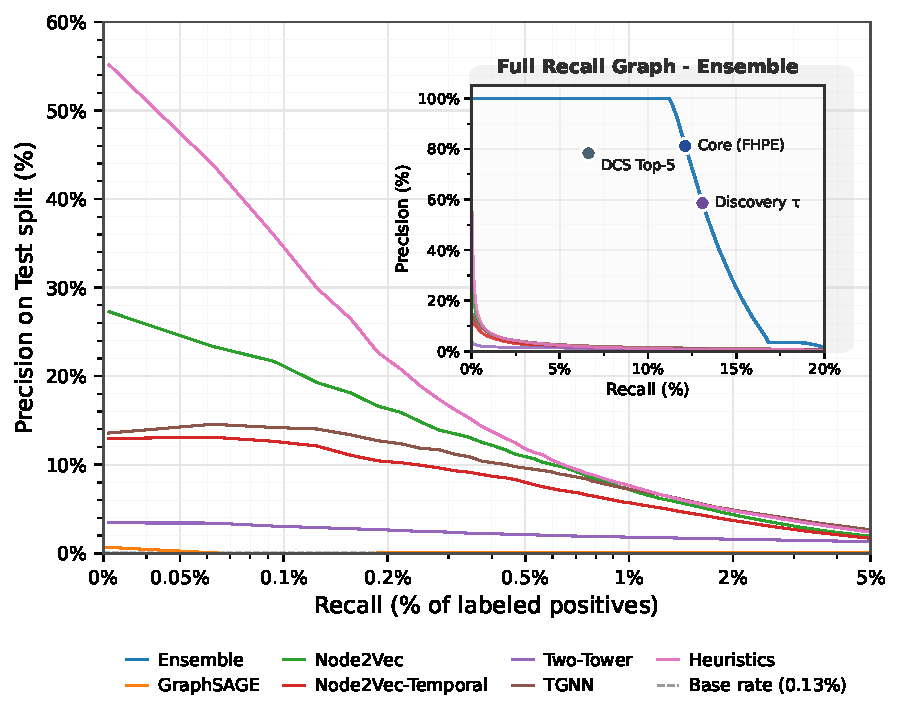
\includegraphics[width=\linewidth]{report/figures/fig_02_pr_curve_test.pdf}
  {
    \captionsetup{justification=raggedright,singlelinecheck=false}
    \caption*{\footnotesize \textit{Note}. {The main panel plots \emph{Precision (\%)} versus \emph{Recall (\%)} on the test split for representative models, \emph{zoomed to the operational regime} where recall is small (typically 0--8\%). Curves use monotone interpolation, so precision is non-increasing in recall. The ensemble (thick line) dominates in the high-precision, low-recall region; a horizontal line indicates the base rate. The inset (upper right) shows the \emph{full recall range for the ensemble} with markers at three operating artifacts: \emph{Core (FHPE)} (high-precision global threshold), \emph{Discovery} (a slightly lower precision target admitting more edges), and \emph{DCS Top-5} (a supplier-balanced subset drawn from FHPE that improves spread by limiting hub dominance). Thresholds for Core/Discovery are chosen on a held-out validation set after probability calibration to meet stated precision targets; markers are placed at the corresponding test precision/recall coordinates. Measured test precision and recall are conservative lower bounds in a positive--unlabeled setting.}}
  }
\end{figure}

The precision--recall curve in Figure~\ref{fig:pr-curve-zoom-inset} also helps explain why the analysis treats the calibrated ensemble as the production model. In the zoomed main panel, the ensemble curve stays at or near \(100\%\) precision out to non-trivial levels of recall. These operating points correspond to very strict probability thresholds that accept only a tiny fraction of candidate edges. Yet, almost all of those accepted edges coincide with labeled positives, despite the extremely low base rate. In such a setting, it is statistically plausible for a well-calibrated model to achieve perfect or near-perfect measured precision at small but meaningful recall, because it concentrates its mass on the most obvious true positives. The strongest single models still fall short of the ensemble in this practically useful region, where recall reaches several percentage points. The horizontal base-rate line lies near the bottom of the plot, reflecting that a vanishingly small share of candidate edges are labeled as positives. The ensemble's curve remains far above this line even when recall increases, which corresponds to many hundreds of times improvement over random guessing at the same yield \parencite{davis_relationship_2006,manning_introduction_2008}.

The inset shows the full recall range for the ensemble and marks three reference operating points that the analysis returns to throughout this section. The first is the \emph{Core} policy, a Fixed High-Precision Ensemble (FHPE) operating point in which the analysis selects a single probability threshold on the validation split to meet a \(95\%\) precision target, then applies that threshold to the test split. \emph{Discovery} is defined in the same way but with a more permissive validation target of \(85\%\) precision, which admits more edges at somewhat lower precision. \emph{DCS Top-5} is a supplier-balanced variant that operates within the Core regime. It defines a Distributed Coverage Subset (DCS) of the FHPE selections by keeping at most 5 accepted edges per source supplier to spread high-confidence links across more firms and avoid concentrating entirely on the largest hubs. Together, these points illustrate the part of the frontier that is relevant for the DoD: a small slice of the curve where precision remains very high, recall is modest but non-trivial, and the model surfaces short lists of candidate links that are plausible enough to merit attention \parencite{hand_measuring_2009}.

The precision--recall view helps in understanding the basic trade-off between precision and recall. For many applications, however, it is more natural to think in terms of the number of edges the analysis is willing to accept. Figure~\ref{fig:precision-yield-frontier-val} expresses the same global-threshold sweep as a precision--yield frontier for the ensemble. The horizontal axis reports yield, the share of candidate edges that clear the threshold, and a secondary axis converts this into the implied number of accepted edges per million candidates. The vertical axis reports measured precision, with a dotted line at the base rate. Each point on the curve, therefore, answers a practical question. If the analysis is willing to accept roughly this many edges, what lower-bound precision can the analysis expect, and how selective is this policy relative to random guessing at the same yield \parencite{manning_introduction_2008,davis_relationship_2006,hand_measuring_2009}?

The three operating points from the precision--recall figure sit on this frontier. The Core FHPE policy lies in a very conservative region. On the test split it delivers about \(\CorePrecision\%\) measured precision, roughly \(12.1\%\) recall, and on the order of \(78{,}981\) accepted edges, with lift of about \(\CoreLift\times\) the base rate. Discovery relaxes the threshold. It yields about \(59\%\) precision, roughly \(13.1\%\) recall, and around \(118{,}235\) edges, with lift still near \(442\times\) the base rate. DCS Top-5 sits below Core in yield because it keeps only five FHPE edges per supplier, but still attains about \(78\%\) precision, roughly \(6.6\%\) recall, and around \(44{,}841\) edges, with lift close to \(591\times\) the base rate. These points trace a small but important segment of the frontier where precision remains high, and the model surfaces tens of thousands of plausible candidate links. That is exactly the regime in which screening for hidden dependencies is feasible and useful for DoD risk assessment \parencite{craighead_severity_2007,pettit_ensuring_2013}.

% ---------------------Precision-Yield Frontier ---------------
\begin{figure}[tbp]
  \centering
  \caption[\textit{Precision-Yield Frontier}]{\textit{Precision-Yield Frontier}}
  \label{fig:precision-yield-frontier-val}

  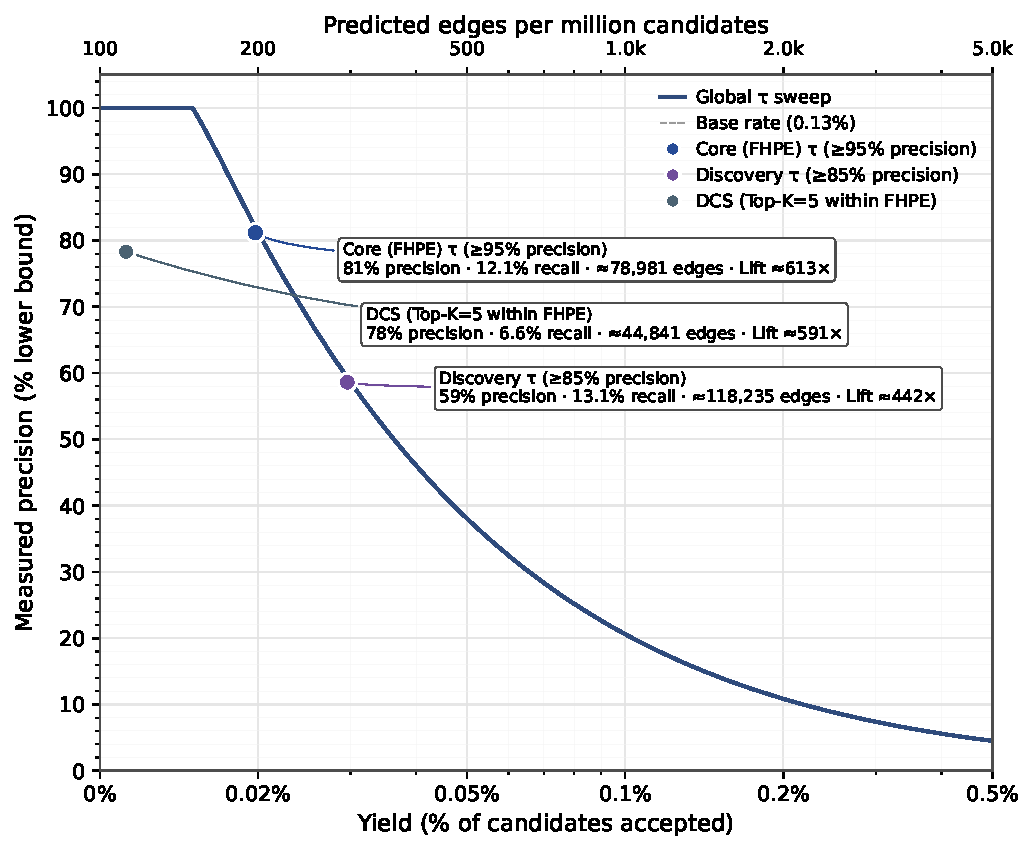
\includegraphics[width=\linewidth]{report/figures/fig_03_precision_yield_frontier_test.pdf}

  {%
    \captionsetup{justification=raggedright,singlelinecheck=false}
    \caption*{\footnotesize \textit{Note}.  The curve traces measured precision (lower bound) against yield (share of candidates accepted), with a secondary top axis showing predicted edges per million candidates.
  Three annotated operating artifacts are highlighted:
  \emph{Core (FHPE)} selected to meet a 95\% validation precision target (test: {\CorePrecision\%} precision, {12.1\%} recall, \(\sim\){78{,}981} edges, lift \(\sim\){\CoreLift}\(\times\));
  \emph{Discovery} at an 85\% target (test: {59\%} precision, {13.1\%} recall, \(\sim\){118{,}235} edges, lift \(\sim\){442}\(\times\));
  and the \emph{DCS} view (Top-\(K{=}5\) within FHPE) for representational coverage ({78\%} precision, {6.6\%} recall, \(\sim\){44{,}841} edges, lift \(\sim\){591}\(\times\)).
  The dotted line marks the base rate (\(\sim 0.13\%\)).
  % Provenance note (kept concise, not a formal citation line):
  Values follow the annotations in the exported figure.
  }
  }
\end{figure}

Global thresholds treat all suppliers symmetrically and are useful for thinking about overall precision and yield. Still, in many settings, they produce a single large, pooled set of inferred links, which is not how people actually work. Program offices, supply-chain analysts, and risk teams often examine specific firms or programs and request a shortlist of ``extra'' dependencies that warrant further review. To reflect that workflow, the analysis also considers a family of per-supplier Top-\(K\)+floor policies. These policies start from the same calibrated ensemble probabilities but differ in how they turn them into decisions. For each source supplier, the analysis ranks its candidate customers by \(p_{\text{meta}}\), keeps only edges whose probability exceeds a floor \(\tau\), and then takes at most \(K\) edges for that supplier. In some variants, the analysis also limits the frequency with which the same destination can appear to avoid concentrating entirely on a few dominant hubs. The result is not a single global list but a collection of bounded shortlists, one per supplier, each containing at most \(K\) high-confidence candidate links.

This construction is analogous to how information retrieval and recommender systems often evaluate the relevance of the top-\(N\) items shown to each user rather than the entire ranking \parencite{manning_introduction_2008,herlocker_evaluating_2004,cremonesi_performance_2010}. Here, the ``users'' are individual suppliers, and the ``recommendations'' are customer relationships that may represent hidden dependencies. In practice, these per-supplier shortlists support analyst-in-the-loop workflows, where a human reviews a few high-confidence candidates for each firm of interest rather than attempting to triage a single global list \parencite{kamar_directions_2016,amershi_guidelines_2019}.

Figure~\ref{fig:heatmap-topk-floor} summarizes the behavior of these Top-\(K\)+floor policies on the test split as a two-dimensional grid. Each row fixes the per-supplier cap \(K\), so moving up or down changes the number of candidate edges each supplier is allowed to contribute. Each column fixes the probability floor \(\tau\), so moving left or right changes how strict the per-edge probability requirement is. Cell shading encodes recall, and each cell is annotated with the exact recall value and the approximate number of accepted edges. Within the region shown in the figure, precision remains uniformly very high because all policies combine relatively tight probability floors with the same calibrated ensemble probabilities that underlie the Core FHPE regime. The main variation across cells comes from the number of true positives and the total number of edges each setting admits.

% ---------------------------- Heatmap ----------------------
\begin{figure}[tbp]
  \centering
  \caption[\textit{Recall for Top-$K$ Policies Across Probability Floors}]%
  {\textit{Recall for Top-$K$ Policies Across Probability Floors}}
  \label{fig:heatmap-topk-floor}

  % Graphic
  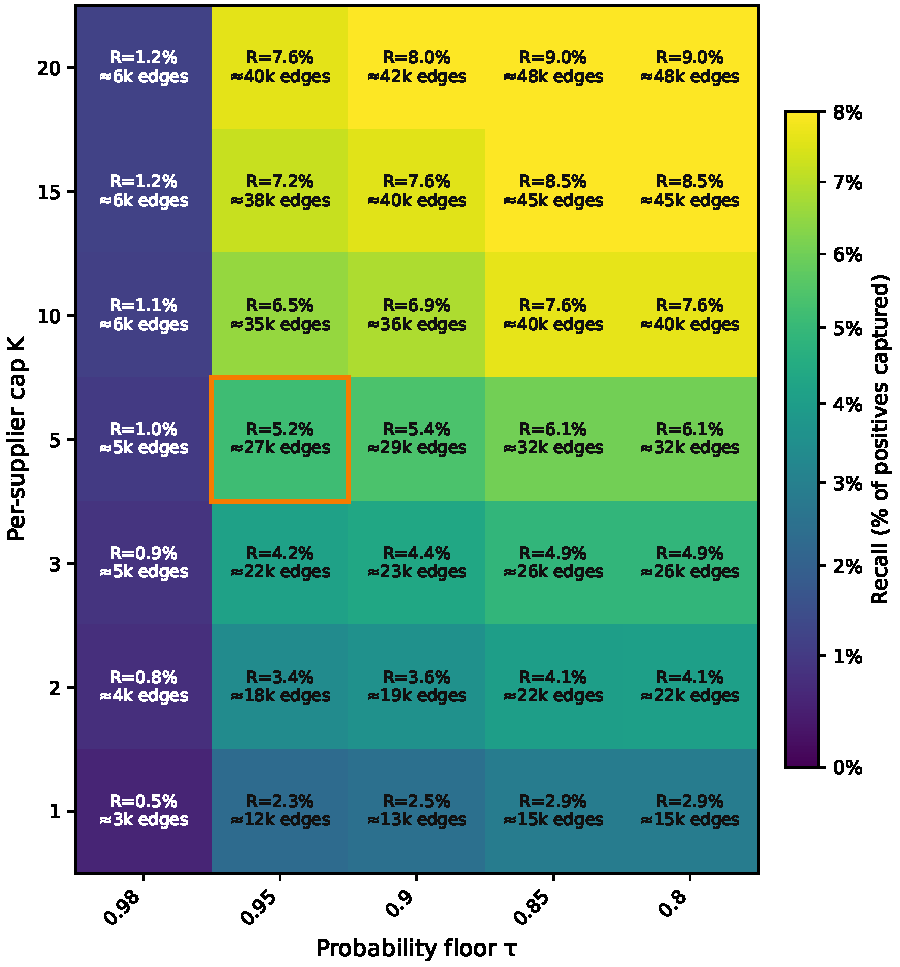
\includegraphics[width=\linewidth]{report/figures/fig_04_topk_floor_heatmap_recall_test.pdf}
  {%
    \captionsetup{justification=raggedright,singlelinecheck=false}
    \caption*{\footnotesize \textit{Note}. {Test-split recall for Top-$K$ plus probability-floor policies. Each row fixes the per-supplier cap $K$ (maximum edges contributed per supplier), and each column fixes the minimum per-edge probability floor $\tau$. Cell shading maps recall---the share of true positives surfaced. Each cell annotates the exact recall value ($R=\cdot\%$) and the approximate number of candidate edges forwarded ($\approx\cdot$ edges). In this operating region, precision remains very high; variation primarily reflects admitted alert volume. The orange outline highlights the \emph{Core (FHPE)} policy at $K=5,\ \tau=0.95$, which emphasizes high precision while bounding supplier dominance. Moving toward the lower-left (smaller $K$, larger $\tau$) reduces both recall and workload; moving toward the upper-right increases coverage at the cost of additional review load.}
  }}
\end{figure}

The orange-outlined cell marks the Top-(K) analogue of the Core FHPE regime, with \(K=5\) and \(\tau=0.95\): at most five inferred links per supplier, and a probability floor matching the high-precision FHPE threshold. This configuration strikes a conservative balance. It allows at most five inferred links per supplier, requires very high predicted probabilities, and, in return, surfaces a moderate number of edges with strong recall under such a strict regime. Moving toward smaller \(K\) or higher \(\tau\) further tightens the policy, reducing both workload and recall. Moving toward larger \(K\) or lower \(\tau\) expands coverage and increases the number of edges forwarded for review, at the cost of greater analyst effort. The heatmap, therefore, provides a visual map of the local tradeoffs around FHPE and helps identify neighboring settings that might be attractive if DoD is willing to shift slightly along the recall--workload frontier.

Up to this point, the analysis has focused on overall precision and yield. For the DoD's purposes, however, the value of an operating point depends just as much on how it behaves in the hardest parts of the graph. Deep-tier dependencies are exactly the links that are structurally distant and weakly connected, so the analysis uses the same selection machinery to report precision, recall, and yield for Core FHPE and Discovery on the structural slices defined in \S2.2. These include cold--cold pairs where both endpoints are unseen in the train window, edges that lie beyond two hops in the train-time graph, and low-degree sources that proxy for smaller or less prominent firms. Across these slices, the high-precision policies retain strong precision and deliver non-trivial recall, even though the task is more demanding than on warm, well-connected nodes. The Core FHPE and DCS Top-5 regimes are particularly important. They do not collapse to trivial behavior that only recovers already-obvious hubs, but instead recover a meaningful number of deep-tier links while keeping measured precision high under conservative positive--unlabeled estimates \parencite{elkan_learning_2008,du_plessis_analysis_2014}. This slice-wise performance is essential for supply-chain risk assessment. The operating points analyzed are those that not only appear good on average but also reveal hidden, structurally remote dependencies that are most likely to drive severe disruptions if they fail \parencite{craighead_severity_2007,pettit_ensuring_2013}.

These operating regimes are a small menu of ways to deploy the ensemble that align with different needs. The Core FHPE policy is the default for high-stakes use. It produces a compact set of inferred links with very high measured precision and substantial lift, suitable for targeted analyst review, due diligence checks on key primes and sub-tiers, and early warning about critical single points of failure \parencite{hand_measuring_2009,craighead_severity_2007,pettit_ensuring_2013}. The DCS Top-5 policy starts from the same Fixed High-Precision Ensemble selections but enforces a strict per-supplier cap. It is designed for coverage-oriented tasks, such as mapping the breadth of the DoD semiconductor supplier base or preparing inputs for structural vulnerability analysis, where the analysis seeks high confidence while avoiding a focus on a handful of dominant firms. The Discovery regime relaxes the precision target and admits more edges. It is most useful for exploratory analysis, including wargaming and scenario design, where analysts are willing to tolerate more false positives in exchange for a richer view of possible dependencies \parencite{hand_measuring_2009,kamar_directions_2016,amershi_guidelines_2019}. In the remainder of the report, the analysis treats Core FHPE and DCS Top-5 as canonical operating points. When the analysis builds the enriched DoD semiconductor network in Section~\ref{chap:dod-supply-chain}, predicted edges are added to the graph only if they are selected under one of these policies, with Discovery-style thresholds reserved for supplementary, explicitly exploratory exercises.

%========================
% Section 2.10
%========================
\section{Robustness, Reproducibility \& Limits}

This section has developed the predictive machinery needed to extend the disclosure graph beyond the edges reported by FactSet. The analysis begins by defining the frozen-core dataset and a leakage-safe training, validation, and test scheme with fixed candidate pools and shared structural and temporal slices. The analysis then introduces a lineup of models ranging from deterministic heuristics to static and temporal learned models, calibrated their scores to comparable probabilities, and stacked them into an ensemble. The scorecards in \S2.8 and the operating-point analysis in \S2.9 show that the calibrated ensemble, evaluated under the Core FHPE and DCS Top-5 operating regimes, is the production predictor for the remainder of the report.

In this final section, the analysis steps back from individual models to focus on robustness, reproducibility, and limits. The analysis documents how the dataset, analysis tables, and scripts are fixed and versioned, summarizes evidence that the main performance patterns are stable across seeds, slices, and horizons, and outlines the most important constraints imposed by the data and modeling assumptions. These choices and limits define the scope of what the analysis can claim when the analysis carries the predicted links into the DoD-focused network construction in Section~\ref{chap:dod-supply-chain}.

Reproducibility in this section begins with the frozen-core dataset defined in \S2.1. The analysis fixes a single snapshot of the SCR event history, canonicalizes overlapping records into a consistent edge timeline, and assigns firms to a deterministic node index. The analysis then constructs leakage-safe train, validation, and test windows with \InterSplitGap-day gaps and builds a train-time snapshot \(\mathcal{G}_{T_0}\) and a matched set of node features. The validation and test candidate pools are fixed in advance and shared across all models, as are the evaluation metrics and structural and temporal slices introduced in \S2.2. Every model in the section is trained and evaluated on the same frozen-core dataset release, with no adjustments to the splits or candidate pools. All headline tables and figures are generated from a small set of analysis tables that record per-edge scores, per-model metrics, and operating-point summaries. The frozen dataset, deterministic splitting scheme, and shared analysis artifacts ensure that the results in this section can be reproduced from the same inputs and that subsequent sections refer to a single, stable data release.

To guard against artifacts from random initialization and sampling, the analysis treats multi-seed training as a basic robustness check. For each learned model family --- Node2Vec, Node2Vec-Temporal, TGNN, GraphSAGE, and Two-Tower --- the analysis first fixes a production hyperparameter configuration on the validation split, then trains five independent models with different random seeds. The heuristic baselines are deterministic (no random initialization); the confidence intervals reported for heuristics in Table~\ref{tab:seed_robustness} reflect variation across the three scoring functions (PA, CN, AA), not across random seeds. The ensemble meta-ranker is fit once on seed-averaged calibrated probabilities from the base models, so its behavior reflects the average performance of the underlying experts rather than a single realization. The main scorecards in \S2.8 report seed-averaged metrics for each learned model, and Appendix~\ref{app:extended-results} summarizes key metrics as a mean with associated dispersion across seeds, along with the number of seeds contributing to each estimate. Across these checks, model rankings remain stable, and the uncertainty bands are small relative to the gaps between model families. The ensemble and temporal models consistently dominate their static counterparts, and the ensemble remains the top overall ranker. This pattern supports confidence that the headline conclusions in this section do not depend on a lucky draw of initialization or mini-batch ordering.

Robustness in this section also means checking that the main patterns hold across different parts of the graph and across time, not just in aggregate. The structural and temporal slices introduced in \S2.2 and reported in the scorecards in \S2.8 show that the ensemble's advantages are largest in exactly the regions that matter most for hidden dependencies. On structural slices, the ensemble and temporal models deliver the biggest gains in cold--cold quadrants, on edges beyond two hops in the train-time graph, and for low-degree sources, all of which proxy for deep-tier and structurally distant suppliers rather than already-visible hubs. On temporal slices, static Node2Vec performs best at very short horizons, while temporal models, especially the TGNN variant, perform best at long horizons. The ensemble combines these behaviors and raises average precision at intermediate and long horizons, where early-warning value is greatest. The operating-point analysis in \S2.9 uses the same diagnostics to evaluate Core FHPE and Discovery at their chosen thresholds and to check that coverage-oriented policies such as DCS Top-5 preserve high precision overall while still surfacing a non-trivial number of deep-tier links. These results indicate that the visibility gains the analysis claims for the ensemble are not limited to easy, warm, short-horizon edges, but extend into the harder parts of the disclosure graph where DoD's blind spots are most acute.

The main limitations of this section stem from the data and label structure rather than any single modeling choice. FactSet SCR provides a selective view of the supply chain, skewed toward larger, more visible firms and relationships that counterparties choose to disclose. Many smaller sub-tier suppliers, certain geographies, and some types of contractual arrangements are likely to be under-represented. The analysis, therefore, frames link prediction as a positive--unlabeled problem in which the analysis observes a subset of true supplier--customer pairs and treats all other candidate edges as unlabeled rather than as confirmed non-edges \parencite{elkan_learning_2008,du_plessis_analysis_2014}.

This decision has three direct consequences for the results in this section. First, all reported precisions are lower-bound estimates, since some edges counted as false positives are almost certainly real but undisclosed relationships. Second, recall is defined only with respect to the set of observed positives in the candidate pools, not with respect to the full, unknown set of true dependencies. Third, the models can only surface firms and edges that enter the candidate construction process. DoD-relevant suppliers that never appear in SCR, or that fail to pass through the entity-resolution and candidate filters in \S2.1, will not be visible to the machinery developed in this section. These are structural limits of the disclosure data and label regime, and they set an upper bound on the completeness of any inferred network.

It is natural to ask whether the relatively modest recall at the chosen operating points is a limitation for the rest of the report. The answer depends on the baseline. The candidate pools in \S2.2 have an extremely low base rate, so even small increases in recall correspond to tens of thousands of additional inferred edges, and the operating points in \S2.9 deliver lifts of several hundred times over random guessing at the same yield. In this setting, the analysis deliberately trades recall for very high precision and a manageable workload, because DoD actors cannot meaningfully review or integrate millions of noisy candidate links. The goal of the modeling is not to recover every missing edge in the global supply chain, but to expand the observable network in a way that is both conservative and useful for screening. As long as the added edges are highly likely to be real supplier--customer relationships and disproportionately concentrated in structurally hard regions of the graph, they can materially change the DoD-relevant network while leaving some residual blind spots. Sections~3 and 4 are designed with this constraint in mind. They treat the inferred edges as high-confidence hypotheses that extend visibility, rather than as a complete reconstruction of the underlying supply chain.

Finally, the models and operating points introduced by the analysis rest on substantive modeling assumptions that shape how their outputs should be used. All the learned models approximate a strategic, evolving supply network by fitting statistical link-prediction rules to historical disclosure patterns. The temporal architectures assume some stability in how and when relationships are disclosed, and the calibration and ensemble weights are estimated on one validation window and then applied forward. The ensemble meta-ranker is deliberately simple and linear in its use of calibrated expert probabilities, which improves interpretability but cannot capture every possible interaction among experts or all forms of distribution shift. The analysis does not claim that these models identify causal dependencies or forecast specific events. They generate ranked hypotheses about plausible supplier--customer links under a conservative positive--unlabeled evaluation, and their outputs are best read as structured inputs to analyst-led investigation rather than as definitive statements about the supply chain \parencite{kamar_directions_2016,amershi_guidelines_2019}.

Section~\ref{chap:dod-supply-chain} shows why this predictive machinery is necessary and how the analysis uses it to construct the DoD-relevant network. The analysis treats the Department as tier zero, uses federal contracting data to establish a factual list of tier-one suppliers, and then expands this graph using disclosed SCR links, observed shipping connections, and high-confidence predicted edges drawn from the ensemble at the operating points defined in \S2.9. The goal is not to recover the full global semiconductor supply chain, but to build an enriched, DoD-anchored network that is substantially more informative than procurement data alone and that provides a defensible substrate for the structural vulnerability and disruption-cascade analysis in the rest of the report.

% ------------------------------------------------------------------
% End of Chapter 2 outline
